\documentclass[14pt,a4paper]{article}
\usepackage[utf8]{inputenc}
\usepackage[paper=a4paper, margin=1.5cm]{geometry}

% FA icons
\usepackage{hyperref}
\usepackage{url}
\usepackage{color}
\usepackage{xcolor}
\usepackage{graphicx}
\usepackage{tikz}
\usepackage{minted}

\setminted{
    breaklines=true,
    fontsize=\footnotesize,
    framesep=2mm
}

\usepackage{caption}
\usepackage{subcaption}

\floatplacement{figure}{H}

\DeclareCaptionLabelFormat{numeric}{příloha #2.}
\captionsetup{labelformat=numeric,labelsep=quad}

\usepackage{amsmath}
\usepackage{amssymb}

\hypersetup{
    colorlinks=true,
    linkcolor=blue,
    filecolor=magenta,      
    urlcolor=cyan,
    pdftitle={Bakalářská práce - Využití IT ke generování zadání písemných testů},
    pdfpagemode=FullScreen,
    colorlinks=false,% hyperlinks will be black
    pdfborderstyle={/S/U/W .5}% border style will be underline of width 1pt
}

% citace a jazyk
\usepackage[main=czech, english]{babel}
\usepackage{csquotes}
\usepackage[style=iso-authoryear]{biblatex}
\addbibresource{zdroje.bib}

\begin{document}
	\begin{titlepage}
		\begin{center}
            {
            \centering
            
\includegraphics[]{./img/UP_logo_PdF-UP_horizont_cz.pdf}
            }
			
			\vspace{3cm}

            {
                \LARGE
                \textbf{Šimon Janča}\\
                3.\,ročník\\[8mm]
                Obor: Informační technologie a Matematika pro vzdělávání
            }

            \vspace{4cm}
			
			{
			    \textbf{\Huge Využití IT ke generování zadání písemných testů}\\[4mm]
			    \Large
			    Bakalářská práce
			}

            \vfill
            
            {
                Vedoucí práce:
                doc. RNDr. Petr Šaloun, Ph.D.
                \hfill
    			Olomouc \the\year{}
            }
			
		\end{center}
	\end{titlepage}
	% generate table of contents
	\tableofcontents

	\newpage
    \clearpage
    \setcounter{page}{1}
	
	\section{Úvod}
    V~úvodu této práce bych~chtěl na~několika stránkách popsat nástroje, které učitelé používají pro~tvorbu písemných prací pro~své~žáky a~definovat potřeby, které v~této souvislosti mohou nastat.
    
    Ve~druhé části popíšu návrh a~implementaci aplikace, kterou by~učitelé k~tvorbě různých variant zadání mohli používat. V~rámci toho bych chtěl popsat základní prvky při~vývoji \textbf{moderní MVC} aplikace a~popsal důvody k~jednotlivým rozhodnutím od~návrhu a~výběru technologií, přes plánování pomocí diagramů, až k~její implementaci a spuštění za~použití vybraných technologií. Pochopitelně nepůjde o~jediný způsob, jak mohou aplikace vzniknout, nicméně by~mělo jít o~čitelný a~reprodukovatelný postup vývoje, zabezpečení a~údržby podobné aplikace. Vyhotovená aplikace bude následně veřejně dostupná jako webová služba.

    \section{Testy, testové úlohy}
    
    Testy jsou~jedním z~nejpoužívanějších nástrojů pro~ověření znalostí žáků. V~dnešní době se~testy používají nejen pro~ověření znalostí, ale i~pro~získání zpětné vazby od~žáků.
    
    Testy mohou být psány ručně, nebo mohou být generovány pomocí počítačových nástrojů. V~této kapitole se~budu zabývat problematikou testových úloh, jejich tvorbou a~možnostmi, které nám dnešní technologie nabízí.

    V~rámci této práce se~budu zabývat především písemnými testy, které jsou~používány na~základních a~středních školách. Nicméně většina z~popisovaných technik je~použitelná i~pro~jiné typy testů.
    
    Součástí práce je~dotazník určený učitelům, který by měl poskytnout informace o~tom, jaké nástroje učitelé v~současnosti používají.

        \subsection{Uzavřené úlohy}
        
        \textbf{Uzavřené úlohy} jsou~úlohy, které mají předem danou množinu odpovědí. Respondendt si~při~vyplňování testu vybere jednu z~nich (nebo více správných, podle zadání) a~tím odpoví na~otázku. Může jít o~označení vyjmenovaných možností nebo z~obecně předpokládaných odpovědí, např.~na~otázku \uv{V~jakém městě bydlíte?} očekáváme v~odpovědi město, nikoliv několik popisných vět.

        Řešení takových úloh může~být~méně náročné, jak na~žáka, který může jednodušeji určit (nebo uhodnout) správnou odpověď, tak na~učitele, který nemusí při~hodnocení brát v~potaz různé možnosti odpovědí.

        Nabízí se~tím možnost zápisu do~odpovědních archů a~tím jednodušší vyhodnocení pomocí počítače.

        Bodování úloh může být jednoduché, kde~za~každou správnou odpověď přičteme jeden bod, nebo může být složitější, kde např.~za~každou správnou odpověď přičteme jeden bod, ale za~každou špatnou odpověď bod (nebo část bodu) odečteme, za~nevyplněnou odpověď většinou nepřičítáme ani~neodečítáme žádný bod.

        Může jít také třeba o~doplnění písmen výběrem za~účelem procvičení správné gramatiky. Také jsou možné různé doplňovačky nebo výběr správného slova do textu, např.~v~cizích jazycích. V~matematice může jít~o~výběr správné hodnoty (nebo množinu hodnot).

        \subsection{Otevřené úlohy}
        \textbf{Otevřené úlohy} naopak předem dané možnosti odpovědí nemají. Respondent musí odpověď napsat sám, odpovědí může být slovo, věta, nebo třeba i~celý text. Může jít o~návodné otázky, kde~je~potřeba odpovědět vlastními slovy, nebo o~otázky, kde~je~potřeba vypočítat nějakou hodnotu a~můžeme zhodnotit odpověď nejen podle výsledných hodnot, ale i~podle postupů, které byly~použity.

        Řešení takových úloh je~náročnější, jak na~žáka, který musí odpověď vymyslet, tak na~učitele, který musí při~hodnocení brát v~potaz různé možnosti odpovědí. Na~druhou stranu to~umožní ocenit i~částečně správné odpovědi nebo vlastní invenci při~řešení, což by~u~uzavřených úloh nebylo možné.

        Může jít o~vypsání odpovědi, nebo třeba výpočet matematického příkladu. \parencite{rozhlasOUtazky}

        \subsection{Tvorba testů}
        Při tvorbě testu ze~začátku uvažujeme o~jeho rozsahu. Jde~o~obecný test, ověřující schopnosti žáka, nebo pouze konkrétního výřezu učiva daného předmětu?

        \uv{Otázky by měly být pestré, pokrývající co nejširší spektrum prověřovaného učiva, a to z různých úhlů pohledu. Takže by určitě neměly chybět otázky zjišťující schopnost žáka pracovat s fakty (značky a jednotky fyzikálních veličin, matematické vyjádření fyzikálních zákonů)}. \parencite{Suchoradsky:testy}
        
        Problémem je~také~tvorba správných a~nesprávných odpovědí při~tvorbě (\emph{uzavřených}) otázek. Pokud naším cílem je~dobře ověřit znalosti, pak~je~nutné tvořit otázky tak, aby nesprávné odpovědi vypadaly věrohodně. Taky nesmíme zapomenout, aby odpovědi obsahovaly správné řešení (může být specifikováni zadáním).

        Můj~druhý obor je~matematika, proto se~v~příkladu zaměřím na~ni. Pokud budeme testovat např.~znalosti \emph{lineárních rovnic}, pravděpodobně necháme otázku s~otevřenou odpovědí, abychom zjistili, zda je~student schopný odpověď vyčíslit. Ale může nastat situace, že~chceme ověřit rychlý úsudek studenta na~základě daného učiva a~pak mu nabídneme možnosti.

        Možnostmi pro~odpovědi k~lineární rovnici budou výsledné hodnoty proměnné (např.~$x$), které můžeme definovat třeba jako násobek jiných koeficientů. Řekněme, že~budeme požadovat, aby výsledek odpovídal některému z~číselných oborů. Pro žáky, kteří neumí počítat se~zlomky budeme chtít rovnici s~celočíselným výsledkem. Naopak pokud chceme ověřit znalost výpočtu kvadratické rovnice s~imaginárními čísly, budeme chtít v~rovnici a v~odpovědích obsáhnout imaginární složku.

        \subsection{V současnosti používané nástroje}
        V~současnosti je~pro~účely tvorby testů používáno několik nástrojů, které se~liší svými možnostmi a~způsobem použití.
        
        Existují některé \textbf{webové stránky}, které nabízejí hotové testy ke~stažení. Ty~potom učitel jen~vytiskne. Na~internetu je~možné najít i~jednotlivé příklady, ze~kterých učitel test sestaví.

        Pokud si~učitel chce test vytvořit, může používat klasické \textbf{tabulkové procesory}, jako je~např.~\textsc{Microsoft Excel} nebo \textsc{Google Sheets}, nebo \textbf{textové procesory}, jako je~např.~\textsc{Microsoft Word} nebo \textsc{Google Docs}.

        V~dnešní době může učitel k~jednoduššímu formátování textu používat formáty \textsc{\LaTeX} nebo \textsc{Markdownu}, který nemá takové možnosti, jako textové procesory třeba MS Word, nicméně umožňují základní formátování textu i~seznamů.

        \subsection{Co na tvorbu testů používají učitelé}
        % TODO: dotazník/rozhovory s učiteli

    \section{Vývoj moderních webových aplikací}
    V dnešní době je~webová aplikace první volbou pro~většinu vývojářů. Je~to~způsobeno tím, že~webová aplikace je~dostupná z~jakéhokoliv zařízení, které má~přístup k~internetu a~je~schopné zobrazit webový prohlížeč. Webová aplikace je~také snadno aktualizovatelná a~není potřeba ji instalovat na~každém zařízení zvlášť, stačí pouze otevřít prohlížeč na~dané adrese.
    
    Vývojáři se~také nemusí starat o~kompatibilitu s~různými operačními systémy, protože webový prohlížeč
    je~dostupný na~většině z~nich. Webová aplikace je~také snadno škálovatelná, protože je~uložena na~serveru a~uživatelé se~k~ní připojují.
    
    Navíc je možné díky různým nástrojům vydat aplikaci pro~různé platformy (Android, IOS\dots) z~jednoho zdrojového kódu.\parencite{adobe:webapp}

    Většina dnešních projektů je~tedy vyvíjena jako~MVC webová \textsc{aplikace}. Tím oddělíme logiku aplikace od~jejího zobrazení, což nám umožňuje vývoj funkční části aplikace nezávisle na~uživatelské části a~můžeme třeba pracovat s~různými technologiemi.
    
    Pro obě části existují připravené technologie, které nám usnadní vývoj a~umožní nám vytvořit aplikaci rychleji a~s~menším množstvím chyb.

    \uv{Pro frontend i backend aplikace existuje na webu obrovské množství použitelných materiálů. Ať už jsou to různé grafické prvky nebo serverové komponenty, to vše je už někde nejspíše hotové.}\parencite{itnetworkBestPractices}

        \subsection{Základní statická HTML stránka}
        V roce 1989 vytvořil Tim Berners-Lee první webový prohlížeč a~jazyk HTML. HTML je~zkratka pro~HyperText Markup Language (Hypertextový značkovací jazyk).
        Základem je HTML stránka~--~soubor, který obsahuje textový obsah a~HTML značky, které určují, význam jednotlivých částí obsahu.
        Navíc lze jednotlivé soubory propojit pomocí hypertextových odkazů, které umožňují uživateli kliknutím přecházet z~jedné stránky na~druhou.

        V dnešní době se~HTML stránky skládají z~HTML značek, ale i~CSS stylů, které určují jak má prohlížeč jednotlivé části stránky zobrazit.
        K tomu se přidává i~JavaScript, který umožňuje přidat do~stránky dynamický obsah a~interaktivitu. \parencite{berners:1989:proposal}

        Jednotlivé prvky je možné také označit pomocí identifikátorů a~tříd, které se~používají pro~jejich identifikaci.
        Zatímco tříd může mít prvek více, identifikátor může mít jen jeden. Identifikátor by měl být unikátní. V jedné HTML stránce by se měl vyskytovat jen jednou.
        Třídy se~používají pro~skupiny prvků, které mají stejný vzhled. Prvek může mít více tříd a~kombinovat tak jejich vlastnosti. \parencite{jpw:tridy}

        \subsection{HTML s dynamickým obsahem}
        HTML stránky mohou mít i~dynamický obsah. To znamená, že~se~mohou měnit podle toho, jak s~nimi uživatel pracuje.
        Na úrovni serveru se~může generovat HTML stránka, která obsahuje dynamický obsah. V~dnešní době se~častěji používá Javascript,
        nicméně v minulosti se~používaly i~jiné technologie, jako např.~\textsc{PHP (HyperText Preprocessor)}, které na~serveru vygenerovaly HTML stránku.

        To samozřejmě znamenalo, že~při~každé změně obsahu bylo~potřeba znovu kontaktovat server a~stránku znovu načíst do~prohlížeče. Také byla veškerá komunikace omezená na~požadavek od~klienta, server pouze obsluhoval požadavky a~neměl možnost samostatně zaslat zprávu klientovi.
        Tento problém právě adresuje Javascript. Odesílá požadavky na~server a~na~základě odpovědi mění obsah celé nebo části stránky. Díky metodám, jako je~\textsc{AJAX (Asynchronous Javascript And XML)}\parencite{ajax:mdn} je~možné komunikovat se~serverem i~bez~načítání celé stránky.
        Server může - samozřejmě po~povolení ze~strany uživatele - zasílat zprávy na~klientské zařízení i~bez~jeho požadavku díky \textsc{Server-Sent Events}\parencite{sse:mdn} nebo udržovat spojení pomocí \textsc{WebSockets}\parencite{websocket:mdn}. Živý přenos videa nebo internetové hovory jsou~příkladem použití WebSockets.

        To~znamená, že~když např.~uživatel klikne na~tlačítko, nemusí se~stránka znovu načítat celá, pouze se~načtou data ze~serveru
        a~přidají se~do~stránky. To~je~rychlejší a~příjemnější pro~uživatele.

        \subsection{Kompilátor a Interpret}
        Pro~lepší pochopení programování aplikací je~potřeba si~ujasnit rozdíl mezi kompilovaným a~interpretovaným jazykem.

        \textbf{Kompilovaný} jazyk je~jazyk, který se~pomocí tzv.\,překladače (kompilátoru) překládá do~binárního souboru, který obsahuje přímo instrukce pro~procesor, které dokáže počítač (procesor) vykonávat. Při~každém spuštění se~do paměti načte binární soubor a~procesor vykonává jeho instrukce.
        
        Při~překladu (\textsc{kompilaci}) překladač navíc kontroluje správnost zápisu a~případné zjistitelné chyby vypíše. To~umožňuje odhalit chyby před spuštěním programu.

        Překladač navíc provádí optimalizace, které zvyšují výkon a~snižují nároky programu.

        \textbf{Interpretovaný} jazyk je~naopak vykonáván programem, kterému říkáme interpret. Ten~čte~příkazy a~přímo je~vykonává. To~znamená, že~při~každém spuštění se~příkazy překládají znovu. Navíc je~interpret program, který musí běžet, zatímco příkazy interpretuje, což je taky jeden z~důvodů, proč bývají interpretované jazyky pomalejší a~náročnější na~využítí zdrojů, než~kompilovaný.
        
        Interpretování může ale přinést i~výhody. Například je~možné příkazy vykonávat ihned, bez~nutnosti překladu a~není potřeba obstarávat správu paměti. \parencite{ueda:compiled}
        
        \subsection{Překladač (kompilátor)}
        Překladač je~program, který čte~zdrojový kód a~překládá ho do~podoby binárního souboru, který obsahuje instrukce vykonávané procesorem. Překladač také kontroluje správnost zápisu a~případné zjistitelné chyby vypíše. To~umožňuje odhalit některé chyby ještě před~spuštěním výsledného programu.
        \textbf{Překladače} i~\textbf{interprety} pracují v~několika fázích:
        \begin{enumerate}
            \item \textbf{Lexikální analýza} - čte zdrojový kód znak po~znaku a~rozděluje kód na~jednotlivé tokeny a~určuje jejich typ (slova, čísla, operátory\dots). Při~tom kontroluje správnost zápisu a~případné chyby vypíše. Výstupem je~seznam tokenů.
            \item \textbf{Syntaktická analýza} - kontroluje, jestli jsou jednotlivé tokeny správně strukturovány a~v~jakém vztahu k~sobě stojí. Generuje \textsc{abstraktní syntaktický strom (AST = Abstract Syntax Tree)}, který reprezentuje strukturu programu.
            \item \textbf{Sémantická analýza} - kontroluje správnost použití jednotlivých tokenů a~jejich význam. Generuje tabulku symbolů, která obsahuje informace o~proměnných a~funkcích, dostupných v~programu.
            \item \textbf{Optimalizace} - v~této fázi optimalizujeme kód, aby byl ve~výsledku rychlejší a~méně náročný na~procesor. Optimalizace se~děje v~závislosti na~použitém jazyce a~překladači a~může být~prováděna několikrát v~různých fázích překladu (a~nemusí být prováděna vůbec).
            \item \textbf{Generování kódu} - Když~máme \textsc{AST}, můžeme generovat výslednou podobu v~požadované formě - binární soubor programu, optimalizovaný bytecode pro spouštění pomocí interpretu, program zapsaný v~jiném jazyce nebo interpretujeme jako~jinou formu dat.
        \end{enumerate} \parencite{baeldungCompilersWork}

        \subsection{Procedurální a~objektově orientované programování (OOP)}
        \textbf{Procedurální programování} je~způsob programování, kdy se~program skládá z~jednotlivých procedur, které se~volají za~sebou. Procedura je~část programu, která vykonává určitou činnost. Procedury mohou mít parametry, které jim předáváme při~volání. Procedury mohou volat jiné procedury, což umožňuje znovupoužití kódu. Procedury a~funkce jsou~si~podobné, kromě faktu, že~funkce vždy vrací (\texttt{return}) nějakou hodnotu, zatímco procedura pouze vykoná své~instrukce. \parencite{procedural:wiki}
        
        V~dnešní době se~častěji používá \textbf{OOP}, protože umožňuje vývojáři programovat v~abstraktnější rovině a~tím zjednodušit vývoj a~údržbu programu. Jednotlivé objekty představují abstrakci objektů z~reálného světa, což~je~pro~člověka přirozenější způsob myšlení. Při~práci v~týmu je~také jednodušší rozdělit si~práci na~jednotlivé části programu, na~kterých mohou vývojáři pracovat paralelně.
        
        \textbf{OOP (Objektově Orientované Programování)} je~programovací paradigma, které se~snaží modelovat objekty z~reálného světa. V~OOP se~program skládá z~objektů, které mají své~vlastnosti a~metody (funkce). \textbf{Objekty} vytváříme ze~tříd, což~jsou jakési vzory, podle kterých se vytvářejí (\textsc{inicializují})~objekty. \textsc{OOP} má 4~základní vlastnosti.
        \begin{itemize}
            \item \textbf{Abstrakce} - třídy mohou být \textsc{abstraktní}, což~znamená, že~nemusí být~implementována jejich funkcionalita a~nelze je~samostatně \textsc{inicializovat}. To~umožňuje vytvářet obecné (tzv.\textsc{bázové})~třídy, které mohou být použity jako vzor pro~odvození jiných konkrétních tříd, využívajících jejich vlastnosti a~metody.
            \item \textbf{Zapouzdření} - objekty mohou své~vlastnosti a~metody, skrýt před~okolním světem. To~umožňuje měnit vnitřní strukturu objektu bez~toho, aniž bychom museli měnit ostatní části programu.
            \item \textbf{Dědičnost} - objekty mohou dědit vlastnosti a~metody od~jiných objektů. To~umožňuje znovupoužití kódu a~zjednodušení programu.
            \item \textbf{Polymorfismus} - objekty mohou mít stejné~vlastnosti a~metody, ale mohou se~lišit v~implementaci. To~umožňuje vytvářet obecné~třídy, které mohou být použity pro~více konkrétních případů.
        \end{itemize} \parencite{Keogh:OOP}

        Jazyk~\textbf{Go} (Golang) podporuje~\textsc{OOP} jen~částečně. Je~nutné si~uvědomit, že~jde o~jazyk \textsc{strukturovaný}, nikoliv \textsc{objektově orientovaný}. Některých vlastností \textsc{OOP} ale můžeme dosáhnout pomocí \textbf{struktur} a~\textbf{rozhrání} (\textbf{interface}). \parencite{go:OOP}
        V~příkladu \ref{oop:difference} je~pro~porovnání ta~samá funkcionalita zapsána v~jazyce \textbf{Javascript} pomocí \textsc{tříd} a~ta~samá funkcionalita v~jazyce \textbf{Go} pomocí \textsc{struktur}, \textsc{rozhraní} a~tzv.~\textsc{receiver function}, což~jsou funkce definované na~dané struktuře. \textsc{Interface} (rozhraní) zajišťují kontrolu, že~na~daném typu~existují požadované metody (\textsc{receiver functions}).
        \textsc{Interface} obecně představují vzor, jakým je~potřeba implementovat budoucí třídy. Výraz \textsc{Interface} obecně definuje komunikaci mezi objekty, viz.~kapitola věnovaná~\textbf{API}

        A \textbf{Javascript} je sice považován za \textsc{objektově orientovaný}, nicméně \textsc{OOP} implementuje formou tzv.~prototypové dědičnosti, nikoliv tradičním použitím tříd. V praxi tak má každý objekt definovanou vlastnost \texttt{proto}, která buďto obsahuje rodičovský objekt nebo obecný prototyp objektů. \parencite[2.1.01]{kantor_javascript}

        \begin{figure}
            \begin{subfigure}[b]{0.45\linewidth}
                \begin{minted}{js}
class Animal {
    constructor(name) {
        this.name = name;
    }

    makeSound() {
        if (!this.sound) {
            const name = this.constructor.name;
            console.log(`What does the ${name} say?`);
            return;
        }
        console.log(`My name is ${this.name} and I go ${this.sound}`);
    }
}

class Dog extends Animal {
    constructor(name) {
        super(name);
        this.sound = "Haf";
    }
}

class Cat extends Animal {
    constructor(name) {
        super(name);
        this.sound = "Mňau";
    }
}

class Fox extends Animal {}

const a = new Dog("Alík");
a.makeSound();
const b = new Cat("Micka");
b.makeSound();
const c = new Fox("Foxy");
c.makeSound();
                \end{minted}
                \caption{Zápis pomocí tříd v Javascriptu}
            \end{subfigure}
            \hfill
            \begin{subfigure}[b]{0.45\linewidth}
                \begin{minted}{go}
import "fmt"

// Animal is an abstract class (interface) in Go
type Animal interface {
	makeSound()
}

// AnimalBase is a base struct to store common properties of animals
type AnimalBase struct {
	sound string
	name  string
}

// Type (struct) representing a dog
type Dog struct {
	AnimalBase
}

// Cat
type Cat struct {
	AnimalBase
}

// Constructor-like function to create an instance of AnimalBase
func NewAnimalBase(name string) *AnimalBase {
	return &AnimalBase{
		name: name,
	}
}

// Method implemented for AnimalBase, which all animals inherit
func (a *AnimalBase) makeSound() {
	fmt.Printf("My name is %s and I go %s\n", a.name, a.sound)
}

// NewDog je tzv. konstruktor objektu Dog, vytvoří v paměti strukturu s konkrétními daty o psovi (jméno) a vrátí ukazatel na dané místo v paměti
func NewDog(name string) *Dog {
	dog := &Dog{
		AnimalBase: *NewAnimalBase(name),
	}
	dog.sound = "Haf"
	return dog
}

// NewCat je konstruktor objektu Cat, vytvoří strukturu s konkrétními daty o kočce
func NewCat(name string) *Cat {
	cat := &Cat{
		AnimalBase: *NewAnimalBase(name),
	}
	cat.sound = "Mňau"
	return cat
}

// a musí implementovat rozhrání (interface) Animal
func animalMakeSound(a Animal) {
    a.makeSound()
}

func main() {
	a := NewDog("Alík")
	animalMakeSound(a)

	b := NewCat("Micka")
	animalMakeSound(b)
}
                \end{minted}
                \label{oop:golang}
                \caption{Stejná funkcionalita v jazyce Go}
            \end{subfigure}
            \label{oop:difference}
            \caption{Zápis OOP v PHP je stručnější než v Go}
        \end{figure}

        \subsection{Javascript}
        Javascript je~skriptovací jazyk, který se~používá k~tvorbě interaktivních webových stránek. Dokáže reagovat na~uživatelské akce, jako je~kliknutí, a~tedy na~rozdíl od~statické podoby HTML stránky dokáže měnit obsah podle toho, jak~uživatel se~stránkou pracuje.

        Vznikl v~roce 1995 a~jeho tvůrci jsou \textbf{Brendan Eich} a~společnost \textbf{Netscape}. Javascript (resp.~Typescript) je~v~současnosti nejpoužívanějším programovacím jazykem na~světě a~používá se~nejen pro~webové stránky, ale i~pro~tvorbu \textsc{nativních} a~dokonce některých \textsc{embedded} aplikací.

        Díky spouštěčům Javascriptu, kterým říkáme \textsc{Javascriptové enginy}, je~možné spouštět Javascript na~různých platformách. A~tak~můžeme Javascript spouštět v~prohlížeči, ale i~na~serveru nebo dokonce na~mikrokontrolerech. Jeden jazyk tak zvládne pokrýt většinu potřeb, které můžeme při~vývoji aplikací mít.

        \textbf{Javascript} dokáže příkazy zpracovávat \textsc{synchronně} (sekvenčně) i~\textsc{asynchronně} (paralelně).
        \textbf{Synchronní} zpracování znamená, že~se~příkazy vykonávají postupně, tak jak
        jsou zapsané.
        \textbf{Asynchronní} zpracování naopak znamená, že~se~příkazy vykonávají nezávisle na~sobě, tedy ke~spuštění dalšího příkazu nečekáme na~dokončení předchozího. To je~užitečné např.~při~načítání dat ze~serveru,
        které může trvat delší dobu. V~tomto případě se~synchronní příkazy vykonávají dál a~když se~data úspěšně načtou, vykoná~se příkaz, který na~ně čeká. \parencite{kantor_javascript}

        Zpracování \textsc{Javascriptu} je~rozdělen do~dvou částí. První částí je~\textbf{Javascriptový engine}, který zpracovává Javascriptový kód a~podle toho spouští instrukce. Druhou částí jsou~tzv.~\textbf{Web APIs}, které poskytuje funkce, které můžeme v~Javascriptu používat, nicméně jde o~instrukce, poskytované nikoliv Javascriptovým enginem, ale prohlížečem. Jde~např.~o~přístupu k~\textsc{DOMu}, kameře, mikrofonu nebo veškeré asynchronní operace, jako je~načítání dat ze~serveru. \parencite{mdn:js}

        \subsection{Typescript}
        Jednou z~nevýhod \textsc{Javascriptu} je, že~není typově bezpečný. To~znamená, že~není možné při~překladu zkontrolovat, zda~jsou všechny proměnné a~funkce použity správně a~jednotlivé typy je~dokonce možné za~běhu měnit. To~může vést k~chybám, které se~projeví až při~spuštění programu, což~je~pro~větší projekty nežádoucí a~proto se~používají jiné jazyky, které typově bezpečné jsou a~po~kontrole jsou přeloženy (kompilovány, transpilovány) zpět do~Javascriptu. Jedním z~nich je~\textsc{Typescript}. Kromě typové kontroly přináší \textsc{Typescript} i~další výhody a~optimalizace, které zjednodušují vývoj a~zvyšují výkon aplikace.

        Typescript přidává do~Javascriptu statickou kontrolu typů, což znamená, že~proměnné mají přiřazený datový typ, který se~během běhu aplikace nemění, což~v~Javascriptu normálně možné je. Díky kontrole typů je~možné provést při překladu kontrolu, zda~jsou všechny proměnné a~funkce použity správně, což redukuje množství chyb. Navíc umožňuje používat nové vlastnosti Javascriptu, které ještě nejsou podporovány ve~všech prohlížečích. A~také umožňuje tvořit vlastní typy a~struktury, které mohou být použity v~rámci \textsc{AJAX požadavků}. Díky tomu můžeme v~\textbf{IDE} (\textsc{Integrated Development Environment}) používat automatické doplňování kódu a~mít tak~lepší přehled o~tom, s~jakými daty budeme pracovat.

        Typescript se~kompiluje (transpiluje) zpět do~Javascriptu a~je~možné při~vývoji v~Typescriptu použít všechny vlastnosti Javascriptu. \parencite[Get started/TypeScript for the New Programmer]{TypeScript}

        \subsection{DOM - Document Object Model}
        DOM je~objektový model dokumentu, který vytváří prohlížeč na~základě HTML kódu stránky. Jednotlivé HTML prvky jsou reprezentovány objekty, tzv.~\textsc{uzly}. Před vykreslením stránky v~prohlížeči, se~nejprve vytvoří DOM, který obsahuje všechny objekty (HTML prvky), které se~mají zobrazit. K~nim pak~prohlížeč přiřadí \textsc{CSS~styly} a~prohlížečové jádro je~vykreslí na~obrazovku. K~DOMu pak můžeme přistupovat pomocí Javascriptu pomocí globálních objektů \texttt{document} a~\texttt{window}.
        
        Díky nim~můžeme aktivně měnit obsah strány, včetně stylů nebo sledovat uživatelské akce a~na~jejich základě spouštět vlastní funkce.\parencite[2.1.01]{kantor_javascript}

        \subsection{React} je~oblíbená knihovna pro~tvorbu \textsc{uživatelského rozhraní}. Je~vyvíjena společností Facebook a~je~používána při~vývoji mnoha webových aplikacích. Je~oblíbená pro svou jednoduchost a~rychlost. Je~také dobře dokumentovaná a~má~velkou komunitu, která ji~podporuje.
        
        React je~postaven na~tzv.\,\textsc{deklarativním} přístupu. To~znamená, že~v~kódu popisujeme, jak má aplikace vypadat, nikoliv jak se~má chovat. To~umožňuje \textsc{Reactu} optimalizovat vykreslování a~zvýšit výkon aplikace.
        
        Existuje mnoho nástrojů, které usnadňují vývoj aplikací v~Reactu, jako např.~\textsc{Create React App} (někdy se setkáme se zkratkou CRA), nebo \textsc{Vite}. Taky je~připraveno spousta již~hotových šablon, komponent a~modulů, které můžeme stáhnout (pomocí `npm`, `yarn`\dots) a~v~naší aplikaci používat.


        Jednotlivé komponenty mohou mít svůj vlastní stav, který se~může měnit. To~umožňuje vytvářet interaktivní aplikace.
        Komponenty mohou být funkcionalní nebo třídní. Funkcionální komponenty jsou jednodušší a~rychlejší na~vytvoření.
        Třídní komponenty jsou složitější, ale umožňují využít všech výhod Reactu. Funkcionální komponenty mohou využívat tzv.~\textsc{React Hooks}, k~dosažení podobné funkcionality, nicméně třídní komponenty jsou stále podporovány a~mohou být použity.
        Navíc \textsc{React Hooks} jsou stále ve~vývoji a~mohou se~změnit.

        Nejnáročnější operace na~výpočetní výkon je~vykreslování webu a~změn v~něm. Tedy změny v~klasickém DOMu.

        React je~díky využití tzv.~\textbf{Virtuálního DOMu} velice rychlý. \textsc{Virtuální DOM} je~kopie DOMu, která se~používá pro~porovnání změn. To~umožňuje aplikaci rozpoznat, kdy je~potřeba reálný~DOM upravit a~kdy ne. Zamezíme tak zbytečným operacím a~zvýšíme výkon aplikace. \parencite{elrom2021react}

        Jednotlivé \textsc{komponenty} mohou obsahovat další (\textbf{vnořené}) komponenty. Tomu říkáme \textsc{zanořování} nebo anglicky \textsc{nesting}. To~umožňuje vytvářet složitější komponenty s~více prvky.
        S~použitím \href{https://react.dev/reference/react/createElement}{\texttt{React.createElement} (viz. dokumentace)} by~takový kód byl složitě čitelný. I~proto máme k~dispozici \textbf{JSX}.

        Při~psaní \textsc{Stavové aplikace} v~Reactu je~taky důležité vědět, že~v~Reactu funguje tzv.~\textsc{One directional data flow} (jednosměrný tok dat). To~znamená, že~data se~předávají směrem z~rodičovské komponenty potomkům, nikoliv naopak. To~umožňuje lepší kontrolu nad~daty, zároveň to~přináší výzvy při~správě stavu aplikace. Proto se~snažíme přesunout zdroj dat, se~kterým pracujeme na~nejvyšší možnou úroveň, aby bylo~možné data předávat do~komponent, které je~potřebují.
        
        Z~toho vyplývá problém zvaný \textsc{prop drilling} (\textsc{rekurzivní předávání dat komponentami}), spočívající v~tom, že~aby se~data dostala k~cílové komponentě, musíme je~předávat přes~několik vnořených komponent, které data třeba vůbec nepotřebují. To~může vést k~tomu, že~se~v~komponentách objeví nepotřebné kódy, které způsobují zbytečnou komplexitu. Při~změně jedné proměnné, která je~předávána přes~několik komponent, je~tedy~potřeba upravit všechny komponenty, které tuto proměnnou používají, abychom data dostali tam, kde~jsou potřeba. To~může být velice nepřehledné a~zdlouhavé.
        
        Při~změně dat dochází také ke~zbytečnému překreslení všech komponent, které data předávají, i~když se~má změna projeviit pouze v~jedné cílové komponentě.

        \textsc{Prop drilling} řešíme tím, že~zdroj dat přesuneme na~nejvyšší možnou úroveň a~na~změny jednotlivých dat upozorňujeme pouze ty~komponenty, které si~je~vyžádají. Tím se~zjednoduší kód a~zvýší se~přehlednost. Navíc se~sníží počet překreslení komponent, což zvýší výkon aplikace.
        
        K~tomu využíváme \textsc{Context API}, který umožňuje vytvořit tzv.~\textsc{kontext} a~zpřístupnit jej~pro~nás v~celé aplikaci. Kontext je~dostupný v~komponentách, které jsou~vnořené v~komponentě, ve~které je~kontext vytvořen. Obvykle \textsc{kontext} vytvoříme v~samostatném souboru pomocí \texttt{React.createContext} a~poté obalíme celou aplikaci pomocí komponenty \textsc{poskytovatele kontextu} (\textsc{provideru}).
        
        Do~kontextu vložíme \uv{obálku} na~data ve~formě \texttt{useState} nebo \texttt{useReducer}. \textsc{Poskytovatel} (\texttt{context.Provider}) pak~do~kontextu ukládá data a~zpřístupňuje je~pro~komponenty, které jsou~vnořené v~komponentě \textsc{poskytovatele}. \parencite{hswolff:reactContextReducer}
        \textsc{Provider} má~vlastnost \texttt{value}, kam vložíme výchozí data, která chceme v~kontextu uchovávat. V~komponentách, které potřebují z~\textsc{kontextu} číst, data načteme pomocí \texttt{useContext}.
        
        Data potom měníme pomocí tzv.~\textsc{reduceru}, což~je~funkce, která jako argumenty přijme stávající stav a~název akce, kterou je~potřeba provést a~na~základě toho vytvoří nový, změněný stav aplikace, který uloží a~upozorní komponenty na~konkrétní změny. Reducer je~obvykle vytvořen spolu s~kontextem v~samostatném souboru a~předává se~jako parametr \textsc{kontextu}. Názvy akcí zapisujeme jako konstanty, které jsou~dostupné v~celé aplikaci. To~umožňuje snadnou změnu názvu akce pro~celou aplikaci najednou. Jelikož porovnání řetězců je pomalejší než porovnání čísel, je vhodné pro~akce používat tzv.~číselníky (\texttt{enum}), které nám poskytuje \textsc{Typescript}. Tím~zajistíme, že~se~názvy akcí ve~výsledné aplikaci reprezentují čísly a~jejich porovnání bude rychlejší. Také nám díky tomu bude \textsc{IDE} lépe napovídat názvy akcí. Dalšími možnostmi řešení stavu je~použití knihoven jako \textbf{Redux} nebo~\textbf{MobX}.

        \subsection{JSX (Javascript XML)} je~rozšíření jazyka Javascript, které umožňuje využívat zápisu komponent jako v~HTML kódu. Jednotlivé prvky jsou tzv.~komponenty, které se~při~překladu (\textsc{transpilaci}) přepisují na~\texttt{React.createElement} a~vykreslují se~do~HTML. To~umožňuje jednodušší tvorbu komponent. \parencite{reactJSX}
        
        Rozdíl práce na~tvorbě komponent za~použití \texttt{React.createElement}, resp.~\texttt{JSX} je~vidět v~kódu~\ref{JSXcomponent}.
        \begin{figure}
            \begin{subfigure}[b]{0.45\linewidth}
                \begin{minted}{js}
function ComponentA({ name }) {
    return React.createElement(
        // typ prvku
        'h1',
        // atributy
        { className: 'greeting' },
        // textový obsah
        'Hello World!'
        );
    }
\end{minted}
\caption{použití React.createElement}
\end{subfigure}
\hfill
\begin{subfigure}[b]{0.45\linewidth}
    \begin{minted}{js}
const App = () => {
    return (
        <h1 className="greeting">Hello World!</h1>
        );
    }
\end{minted}
\vspace{1cm}
\caption{použití JSX}
\end{subfigure}
\label{JSXcomponent}
\caption{Rozdíl použití React vs.~JSX}
\end{figure}

\textbf{Vite} je~nástroj pro~rychlé nastartování projektu nejen v~Reactu ale třeba i~ve~Vue a~\textsc{Vanilla Javascriptu} nebo~\textsc{Typescriptu}. Je~vyvíjen společností \textsc{Vue.js}, která je~známá díky svému frameworku \textsc{Vue.js}, který je~podobný Reactu.

\textsc{Vite} zrychluje spouštění aplikace a~zjednodušuje práci díky tzv.~\textsc{hot reload}, což znamená, že~se~při~každé změně kódu \textsc{frontendu} se~aplikace v~prohlížeči automaticky načte znovu s~novými změnami, bez~nutnosti manipulace s~prohlížečem.

\textsc{Vite} údajně také zrychluje sestavení modulů~--~spojení importovaných modulů do~jednoho výstupu.\parencite{vitejs}

\subsection{Server Side Rendering (SSR) a Static Site Generator (SSG)}
Přestože je \textsc{React} velmi rychlý, zejména díky použití \textsc{Virtuálního DOMu}, je~při~načítání aplikace v~prohlížeči stále nutné počkat, než se~stáhnou, načtou a~provedou skripty, teprve potom se~vygeneruje výsledný \textsc{HTML} obsah a~prohlížeč stránku vykreslí (\textbf{Client Side Rendering~--~CSR})\parencite{mediumWhatCSR}. To~může být problém, pokud máme rozsáhlou aplikaci, která obsahuje mnoho komponent nebo rozsáhlou logiku, kde celý proces může trvat delší dobu a~uživatel musí déle čekat, což~je~samozřejmě nežádoucí.

To~je~možné řešit pomocí metod \textbf{Static Site Generator (SSG)} a \textbf{Server Side Rendering (SSR)}.

\textbf{Static Site Generator (SSG)} je~způsob zrychlení webů, kde generujeme statické soubory webu z~dat, které načítáme z~dynamického zdroje, např.~\textbf{CMS~--~Content Management System (Redakční Systém)}. Data jsou načítána pluginem a~z~nich~jsou - podle předdefinované šablony - generovány statické soubory. Díky tomu, že~jde o~čistě statický obsah, bez~nutnosti \textsc{AJAX} požadavků nebo dynamického generování, je~tento postup rychlostí na~stejné úrovni jako~poskytování statických souborů \textsc{Webovým Serverem}. To~samozřejmě nevylučuje použití \textsc{AJAXu}, ale ten~je~použit na~jiné uživatelské akce, nikoliv k~načítání prvotního obsahu.
Uživateli posíláme statický \textsc{HTML~soubor}, který se~vykreslí před~zpracováním \textsc{Javascriptu} a~mnohem rychleji než~\textsc{Javascriptová} aplikace, které by~HTML nejdříve generovaly a~tím~oddálily vykreslování prohlížečem. Následně na~vygenerované \textsc{komponenty} aplikujeme jejich logiku a~akce. Tomuto procesu říkáme \textbf{hydratace} (\textbf{Hydration}).


\textbf{Server Side Rendering (SSR)} má~koncept podobný \textsc{SSG}, jen na~straně serveru běží naše aplikace, která průběžně (při~změně v~datech) vygeneruje statický obsah s~použitím naší aplikační logiky. Při~prvním požadavku na~aplikaci server zasílá \textsc{HTML} kód celé stránky a~po~provedení \textbf{hydratace} aplikace funguje normálním způsobem. To~umožňuje vytvořit aplikaci, která se~načte rychleji a~přitom neztratíme výhody frameworku, který používáme (např.~React). \parencite{uc:ssrandssg}

Takto vygenerujeme \textsc{HTML kód} (se~skripty ap.) pro~každou stránku pouze v~případě změny obsahu a~uživateli a~uložíme si~jej. Při~dalším spuštění potom načítáme statický obsah, což~ušetří výkon na~straně serveru i~klienta.

\subsection{Client-Server}
Vývoj webových aplikací je~založen na~modelu klient-server.

\textbf{Server} je~počítač, který poskytuje služby klientovi. V~případě webové aplikace je~to~server, který poskytuje HTML stránku, styly a~skripty.
Taky posléze poskytuje data, která se~do~ní načítají a~ovlivňují její obsah.

        \textbf{Klient} je~počítač, který služby serveru využívá. V~případě webové aplikace je~to~webový prohlížeč, který zobrazuje HTML stránku.
        V~případě mobilní aplikace je to~aplikace, která se~spouští na~mobilním zařízení a~komunikuje se~serverem. Např.~messengery, sociální sítě. \parencite{ClientServer}
        
        \textbf{Klient} může být webový prohlížeč, ale i~jiná, např. mobilní aplikace, která posílá požadavky a~data na~server.

        \subsection{Webová služba, webový server}
        Webová služba je~program, který běží na~serveru a~poskytuje data klientovi. Na serveru může běžet více webových služeb, rozlišují se portem, na~kterém běží a~přijímají instrukce a~data. Např.~webová služba HTTP, která poskytuje webová data a~soubory poběží na~portu~80, resp.~dneska hlavně~443 (\textbf{HTTPS}). Další služby mohou být např.~emailová služba SMTP (\textsc{Simple Mail Transfer Protocol}), která poběží nejčastěji na~portu~25 a další.
        
        Služby \uv{naslouchají} na svých portech a~přijímají požadavky od~klientů. K~serverům na~internetu se~přistupuje pomocí \textsc{IP~adresy} a~ke~službám pak~pomocí portu, na~kterém běží. \parencite{webserver:mdn}

        \subsection{DNS - Domain Name Server}
        \textsc{DNS} je~zkratka pro~\textsc{Domain Name Server}, někdy \textsc{Domain Name System}. Je~to~systém, který překládá doménová jména na~IP adresy. To~umožňuje, aby~uživatelé používali lidem čitelná doménová jména namísto \textsc{IP~adres} cílového serveru, které jsou pro~uživatele těžko zapamatovatelné.
        
        Bez \textsc{DNS} by~se~např.~oblíbený český vyhledávač \texttt{Seznam.cz} proměnil ve~směsici čísel \texttt{77.75.79.222}, což~by~uživatel moc neocenil. To~samé by~platilo i~pro~ostatní weby.

        \textsc{Doménové jméno} je~složeno ze~tří částí. První část je~\textsc{subdoména}, která je~volitelná. Druhou částí je~\textsc{doména} (2.\,řádu), která je~povinná a~třetí část je~\textsc{doménová přípona} (TLD, doména nejvyššího řádu), která je~také povinná. TLD mohou být např.~\texttt{.com}, \texttt{.cz}, \texttt{.eu}, \texttt{.org}. Doménové jméno je~v~procesu \textbf{DNS resolve} přeloženo zpět na \textsc{IP adresu}. \parencite{tld:mdn}
        
        \begin{figure}
            \centering
            \begin{tabular}{l l l l l}
                \textcolor{red}{\texttt{protokol}} &
                \textcolor{blue}{\texttt{subdoména}} &
                \textcolor{green}{\texttt{doména}} &
                \textcolor{orange}{\texttt{TLD}} &
                \textcolor{purple}{\texttt{?query}}\\

                \textcolor{red}{\texttt{https}}:// &
                \textcolor{blue}{\texttt{robot}} &
                . \textcolor{green}{\texttt{killermachine}} &
                . \textcolor{orange}{\texttt{com}} &
                / \textcolor{purple}{\texttt{?znicitlidstvo=false\&parametr=42}}
                
            \end{tabular}
            \label{slozeni-uri}
            \caption{Složky URI}
        \end{figure}

        \textbf{DNS Resolve} je~proces překladu doménového jména na~IP adresu. Když si~uživatel vyžádá nějaké doménové jméno, prohlížeč se~připojí k~\textsc{DNS} a~požádá ho o~překlad doménového jména na~IP adresu. \textsc{DNS} odpoví IP adresou, kterou prohlížeč použije pro~navázání spojení se~serverem.

        Když~zadáme do~prohlížeče doménové jméno, prohlížeč se~pokusí najít \textsc{IP~adresu} v~DNS cache, kam si~ukládá již navštívené weby. Pokud adresu nenajde, připojí~se k~nejbližšímu DNS serveru a~požádá jej o~překlad doménového jména na~IP adresu. DNS odpoví IP adresou, kterou prohlížeč použije pro~navázání spojení se~serverem.

        Nejbližší \textsc{DNS} bývá poskytovatel internetu, který si~udržuje \textsc{DNS-cache}, kde~jsou uloženy \textsc{IP} adresy pro~servery, na~které v~minulosti zákazníci přistupovali. Pokud~tedy záznamy ještě nejsou v~\textsc{DNS cache} prohlížeče, zeptá se~prohlížeč poskytovatele (dále \textsc{ISP}), resp.~zašle požadavek na~adresu nastaveného \textsc{DNS}. Pokud ani~potom záznamy v~\textsc{cache} nezíská, požádá o~ně~postupně nadřazený \textsc{DNS}, správce národní domény (\textbf{CZ.NIC}) a~kořenový DNS server.

        \textbf{DNS Záznamy} může upravovat vlastník domény prostřednictvím \textsc{doménového registrátora}. To~umožňuje přesměrovat doménu na~jiný server, nebo~přidat další záznamy, jako např.~\textsc{TXT}, které se~používají pro~ověření domény pro~e-mailové servery, nebo \textsc{MX} záznamy, které používá e-mailová služba pro doručování e-mailů.\parencite{dns:mdn}

        \subsection{Webový server}
        Webový server se~stará o~odpovědi na požadavky, většinou přicházející na~port 443 (\textsc{HTTPS}), dříve port 80 (\textsc{HTTP}).

        Server dostane požadavek ve~formě URL (\textsc{Uniform Resource Locator}, někdy taky \textsc{Uniform Resource Identifier}), která obsahuje cestu k~požadovanému zdroji (souboru/službě).

        Webový server už~neslouží pouze k~poskytování statických souborů, ale i~k~poskytování dynamických dat.

        Může například zajistit, že~se~před odesláním soubor na~serveru zpracuje (např. pomocí PHP) a~do~něj se~vloží aktuální data, nebo před odesláním provést kompresi dat, což uspoří mobilní data a~klient, který přistupuje přes mobilní síť, vám bude vděčný. Na~straně klienta se~pak data rozbalí a~zobrazí.

        Webový server je~také zodpovědný za~směrování doménových jmen ke~konkrétním datům na~daném serveru. To~znamená, že~na~jednom serveru může běžet více webových služeb na~různých doménách.
        Pomocí metody~\textsc{Proxy~pass} můžeme také přesměrovat celý provoz domény na jiný port (např.~na~naši aplikaci). \parencite{webserver:mdn}

        Příkladem webového serveru může být \textbf{Apache}, \textbf{Nginx}, \textbf{Lighttpd}, \textbf{Caddy} nebo \textbf{IIS}\dots

        
        \subsection{MVC - Model View Controller}
        Nejvýznamnějším bodem vývoje aplikací bylo rozšíření architektury \textbf{MVC}. \textbf{MVC} je~zkratka pro~\textbf{Model View Controller}. Podle této architektury oddělujeme logiku aplikace od~jejího zobrazení. To~umožňuje vývoj funkční části aplikace nezávisle na~jejím zobrazení.

        Díky tomu můžeme mít jednu aplikaci, která bude mít různá zobrazení, ale čerpá pouze z~jednoho zdroje. Např.~webová stránka, mobilní i~desktopová aplikace mohou využívat téže~(\textsc{Backend}).

        Má tři složky; \textbf{Model}, který se~stará o~manipulaci s~daty, \textbf{Controller}, který říká \textbf{Modelu}, co~má~dělat a~\textbf{View}, který se~stará o~výsledné zobrazení dat. \parencite{MVC}

        \subsection{Frontend, Backend}
        Dnešní aplikace se~díky architektuře \textsc{MVC} běžně dělí na~\textbf{frontend} a~\textbf{backend}, které pracují spolu, ale jsou oddělené.

        Díky \textbf{MVC} je~takto možné vývoj aplikace rozdělit mezi tým~vývojářů, kde každý může pracovat na~jiné části aplikace a~každá část aplikace má~své rozhraní, takže mohou pracovat téměř nezávisle na~sobě.

        \textbf{Frontend} je~část aplikace, kterou vidí uživatel. Může to být např.~prostřednictvím prohlížeče. Stará se~o zobrazení (\textsc{View}) a~interakci s~uživatelem (\textsc{Controller}) a~komunikuje s~\textbf{backendem}, zejména pomocí asynchronních požadavků na~server. Je~napsán většinou v~HTML, CSS a~Javascriptu.

        \textbf{Backend} je~část aplikace, která běží na~serveru a~zpracovává nebo~poskytuje data \textbf{frontendu}. Spolupracuje s~databází (\textsc{Model}em), souborovým systémem a~dalšími službami, které jsou potřeba pro~fungování aplikace. \textbf{Backend} může být napsán v~různých jazycích, např.~PHP, Java, C\#, Go, Javascript, C++\dots

        \subsection{JSON - Javascript Object Notation}
        \textsc{JSON}~je~formát pro~uložení strukturovaných dat. Je~to~textový formát čitelný pro~člověka i~pro~stroj. Používá se~ke~strukturovanému ukládání a~přenosu dat. Dříve byl~hojně využíván formát \textsc{XML} (\textsc{Extended Markup Language}, který je~podobný struktuře \textsc{HTML}. Ostatně \textsc{XML} stále používá spousta aplikací, zejména aplikace státní správy.

        Formát \textsc{JSON} je~podobný zápisu objektů v~Javascriptu. Obsahuje dvojice klíč-hodnota, které jsou odděleny dvojtečkou. Klíčem je~řetězec, který obvykle popisuje, jaká data jsou v~něm uložena, a~hodnota může být číselná, textová, logická hodnota, pole nebo další vnořená struktura dat.
        
        Práce s~formátem \textsc{JSON} je~pohodlnější než s~formátem XML, protože je~mnohem jednodušší a~čitelnější a~vyžaduje méně kódu, jak na~straně serveru, tak na~straně klienta a~jde~celkově o~úspornější formát.

        \subsection{AJAX - Asynchronous Javascript Request}
        \textsc{AJAX} je~technologie, která umožňuje asynchronní komunikaci, např.~mezi frontendem a~backendem.

        To~znamená, že~při~každém požadavku na~server se~stránka nemusí znovu načítat, ale použije se~\textsc{AJAX}, čímž se~načtou požadovaná data ze~serveru a~změní se~ve~stránce.

        Funkce Javascriptu, umožňující asynchronní požadavky na~server, jsou \texttt{fetch} a~\texttt{XMLHttpRequest}. AJAX využívá různé HTTP metody, jako GET, POST, PUT, DELETE, PATCH. Tyto metody se~používají pro~odlišení typu požadavku.\parencite{ajax:mdn}

        \subsection{API - Application Interface}
        \textsc{API} je~rozhraní, které umožňuje komunikaci mezi~aplikacemi nebo~i~s~hardware. V~případě webových aplikací se~jedná o~rozhraní mezi frontendem a~backendem. Některá rozhrání umožňují taky komunikaci na~stejném zařízení nebo mezi aplikacemi na~různých zařízeních.
        
        Někerá \textsc{API} jsou veřejná a~umožňují komunikaci s~aplikacemi třetích stran. Např.~\textsc{API} Google Firebase, Microsoft Azure nebo Amazon Web Services umožňují tvorbu tzv.~Serverless aplikací, kde~vývojář tvoří pouze \textsc{frontend} a~o~zbytek se~stará externí služba. To~umožňuje vývojářům se~soustředit na~vývoj aplikace a~nemusí se~starat o~infrastrukturu, která je~potřeba pro~běh aplikace.

        V~dnešní době jsou nejrozšířenější formou tzv.~\textsc{REST API} a~\textsc{GraphQL}. Pro komunikaci mezi interními aplikacemi se~často používá \textsc{SOAP}. Různý hardware používá k~ovládání např.~\textsc{UART} a~\textsc{SPI}.

        Velice oblíbená je~metoda \textsc{gRPC} (\textsc{Google Remote Procedure Call}), která je~založena na~protokolu HTTP/2 a~používá binární formát \textsc{Protocol Buffers}. \textsc{RPC} je~zkratka pro~\textsc{Remote Procedure Call} a~funguje tak, že spouští vzdálené funkce, které jsou na~serveru.
        
        Výhodou je, že~gRPC zastává deklarativní přístup, kde definujeme služby a~jejich rozhraní a gRPC vygeneruje pomocný kód pro~jazyk, který používáme. Taky je~díky efektivnější komunikaci rychlejší než~jiné~přístupy. Bohužel je~k~jeho použitínutné se~naučit novému přístupu a~jazyku definice služeb \textbf{protobuf}. \parencite{thenewstackBuildRealWorld}

        \subsection{REST - Representational state transfer}
        \textbf{REST} je~architektura, která definuje způsob komunikace mezi klientem a~serverem. V dnešní době je~díky své jednoduchosti a~rozšířenosti nejčastěji používanou architekturou pro~tvorbu webových rozhrání. Jednoduchost spočívá zejména v~tom, že~každý \textsc{Endpoint} má~svou~vlastní adresu.
        
        \textsc{REST} je~bezstavový, takže každý požadavek je~nezávislý na~předchozím, server si~neukládá data v~závislosti na~připojeném klientovi. To~umožňuje jednodušší testování a~ladění aplikace. Také to~ale~přináší některé výzvy a~omezení, které je~potřeba řešit. Proto je doporučeno omezit využití ukládání dat vázaných na~konkrétní relaci, nicméně nástroje typu \texttt{Cookies} nebo \texttt{Session} je~možné využívat.
        
        \textsc{REST} definuje, jaké \textsc{HTTP metody} se~používají pro~komunikaci, a~každé přiděluje určitý význam. Mezi nejčastěji používané metody patří \textbf{GET}, \textbf{POST}, \textbf{PUT}, \textbf{DELETE} a \textbf{PATCH}. Metoda je~uložena v~hlavičce HTTP požadavku.

        Funkce jednotlivých \textsc{HTTP metod} jsou:
        \begin{itemize}
            \item \textbf{GET} slouží pro~získání dat ze~serveru,
            \item \textbf{POST} pro~odeslání dat na~server,
            \item \textbf{PUT} pro~úpravu dat na~serveru,
            \item \textbf{DELETE} slouží pro~smazání dat ze~serveru,
            \item \textbf{PATCH} potom pro~úpravu části dat na~serveru.
        \end{itemize}

        Souhrnně těmto operacím říkáme \textsc{CRUD operace}, což je~zkratka pro~\textbf{Create}, \textbf{Read}, \textbf{Update} a \textbf{Delete}.

        Kromě požadavků \textbf{GET} se v~těle požadavku posílají data v~textové formě, např.~formátu~JSON. 
        V~případě požadavku \textbf{GET} se~data vkládají do URL adresy, nejsou šifrována a~mají limitovanou velikost maximální délkou \textsc{URL adresy}.

        \subsection{GraphQL}
        Naproti \textsc{REST}u má \textsc{GraphQL} pouze jeden \textsc{endpoint}. \textsc{GraphQL} je~jazyk, který umožňuje klientovi specifikovat, jaká data chce klient získat. To~umožňuje získat všechna potřebná data v~jednom požadavku, což může být výhodné, pokud máme pomalé připojení nebo~při~mobilním připojení, kdy chceme co~nejvíce ušetřit data a~snížit počet požadavků na~server.

        Na~druhou stranu je~implementace \textsc{GraphQL} složitější než~implementace \textsc{REST}, protože je~potřeba implementovat \textsc{GraphQL} server, který bude umět zpracovat požadavky od~klienta. Každý kousek informace, který chceme zpřístupnit, navíc musíme specifikovat v~\textsc{GraphQL} schématu a~vytvořit pro~něj tzv.~\textsc{resolver}, který zpracuje požadavek a~vrátí data. To~zároveň vytváří větší zátěž na~serveru, protože musíme pro~každou vyžadovanou položku spustit vlastní funkci, což~je v~případě větších datových objektů a~přístupů do~databáze neefektivní.

        \subsection{Zabezpečení}
        Vystavením aplikace na~internetu uvádíme naše \textsc{API} do~nebezpečí útoku a~prolomení zabezpečení. Proto je~potřeba aplikaci zabezpečit a~v~žádném případě nespoléhat na~neprůstřelnost zabezpečení knihoven 3.\,stran, které používáme.
        
        To~znamená, že~je~potřeba zabezpečit \textsc{API}, databázi a~další služby, které aplikace využívá. Je~nutné zvážit např.~jaké služby potřebujeme veřejně dostupné a~ke~zbytku služeb zamezit přístup z~internetu pomocí firewallu, ke~službám, ke~kterým potřebujeme soukromý přístup, přistupovat pomocí tzv.~\textbf{SSH tunelu}, ideálně pomocí \textbf{SSH klíče}. Taky je~nutné udržovat systémy aktuální s~nejnovějšími bezpečnostními aktualizacemi.
            
        \subsubsection{Hashování (Hashing)}
        \textbf{Hashing} je~proces, při~kterém ze~zadaných dat použitím určitého algoritmu vytvoří řetězec jiný, tak, že~z~něj nelze získat původní data. To~využíváme např.~při~ukládání hesel, kdy heslo uživatele neukládáme v~původní čitelné podobě, ale jako \textsc{hash}. Při~přihlášení pak~aplikujeme stejnou \textsc{hashovací} funkci na~zadané heslo a~porovnáme ho~s~uloženým \textsc{hashem}. Pokud se~shodují, uživatel je~přihlášen.
        
        Pokud se~někomu podaří z~\textsc{hashe} získat původní data (heslo), nebo dokáže najít jiná data, která po~aplikování algoritmu generují stejný \textsc{hash}, považujeme algoritmus za~prolomený a~měli~bychom ho~přestat používat.
        
        K~\textsc{hashování} hesel navíc používáme tzv.~\textbf{salt (sůl)}, což~je~náhodně vygenerovaný řetězec, který přidáme k~heslu před \textsc{hashováním}. Protože pro~každou kombinaci by~měl algoritmus generovat jiný \textsc{hash}, je takto ztíženo zjištění původního hesla i~v~případě úniku \textsc{hashe}.
        
        \subsubsection{Šifrování (Encryption))}
        U~šifrování naopak potřebujeme získat původní data z~šifrovaného textu. K~šifrovacímu algoritmu potřebujeme klíč, kterým se~šifrují i~dešifrují data. Algoritmu zadáme klíč a~data, která chceme zašifrovat, a~ten nám~vrátí šifrovaný text. Při~dešifrování zadáme algoritmu klíč a~šifrovaný text a~algoritmus nám~zpřístupní původní data.

        Z~hlediska zabezpečení webové aplikace pak~hovoříme o~dvou základních bodech. \textbf{Autentikace} a~\textbf{autorizace}.

            \subsubsection{Autentikace (Authentication)}
            \textbf{Autentikace} je~proces ověření identity uživatele. To~znamená, že~uživatel musí dokázat, že~je~tím, za~koho se~vydává. To~se~dělá pomocí hesla nebo pomocí certifikátu, který uživatel má.
            
            V~případě \textsc{API} se~jedná o~ověření, že~požadavek přišel z~naší aplikace a~ne z~jiného zdroje, např.~od~útočníka. Na~to~existují různé metody, např.~využití \textsc{JWT}.
            
            Do~frontendu aplikace vložíme dvojici tajných údajů, které backendu řeknou, že~jde skutečně o~naši aplikaci, resp.~o~jinou aplikaci, která má~k~backendu přístup. Taky můžeme přístup pomocí tajných údajů omezit na~konkrétní IP adresu, ze~které se~připojuje, nebo jakékoliv další informace, které jsou stálé a~můžeme je~vyčíst z~přicházejícího požadavku.

            Při autentikaci aplikace je~důležité kontrolovat také jestli~požadavek přišel z~povolené IP~adresy, byl vytvořen naší aplikací na~našem webu, klientovu \textsc{IP~adresu} a~další informace, které by~mohly odhalit nepovolený přístup. Při~každém požadavku je~pak potřeba ověřit, že~\textsc{token} nebyl změněn a~přichází stále z~naší aplikace. \parencite{graham2021ethical}
            
            \subsubsection{Autorizace (Authorization)}
            Autorizace je~proces ověření oprávnění uživatele. Ověřujeme, zda~má~uživatel oprávnění k~provedení určité akce, např.~smazání příspěvku.
            To~je nutné ověřit pomocí rolí, které uživatel má, nebo pomocí oprávnění k~operacím s~daným zdrojem.

            Třeba, zda je~uživatel autorem příspěvku a~tedy jej může upravit, pozměnit nebo smazat. \parencite{graham2021ethical}

            \subsubsection{JWT - JSON Web Token}
            Metoda zabezpečení, která se~často používá, je~JWT. Jedná se~o~formát textového řetězce (tokenu), který obsahuje informace o~uživateli a~aktivním stavu aplikace. Ten se~při~každém požadavku posílá v~hlavičce požadavku a~umožňuje tak ověřit, že~požadavek přišel z~naší aplikace a~ne z~jiného zdroje.
            
            Při autentikaci se~vygeneruje \textsc{token} (řetězec znaků), který se~při~každém požadavku na~server posílá v~hlavičce požadavku. Data v~tokenu jsou zašifrována a~podepsána privátním šifrovacím klíčem, takže je~nelze, bez~znalosti klíče, změnit. Do~tokenu se~přidávají data, která potřebujeme uchovat nebo je~využíváme na~dodatečnou kontrolu. V~případě změny nebo nepřesnosti v~datech tokenu se~token stává neplatným. To~umožňuje ověřit, že~token byl vytvořen serverem a~ne někým jiným. Zároveň v~datech tokenu můžeme mít informace o~uživateli, který je právě přihlášen, a~další kontrolní informace, jako např.~\textbf{čas platnosti} tokenu nebo \textbf{IP~adresa} a~\textsc{doména}, ze~které byl požadavek na vytvoření tokenu prvně odeslán.

            Funkci \textbf{JWT} v~praxi lze~vidět na~schématu \ref{model-jwt}.

            \begin{figure}
                \centering
                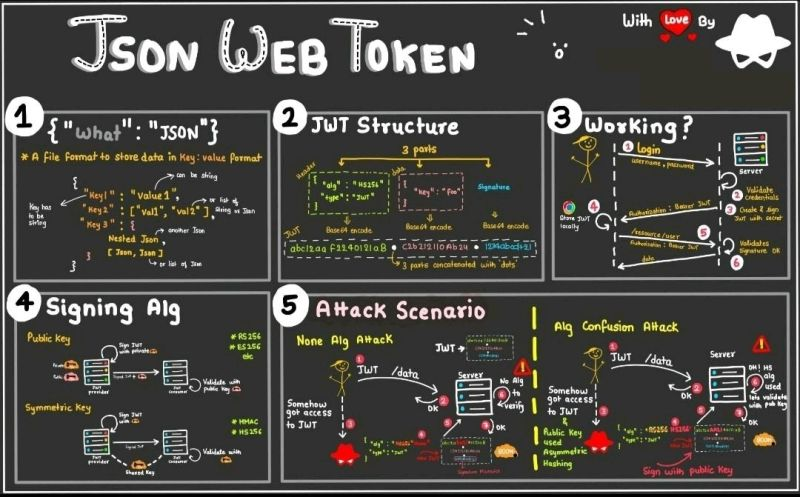
\includegraphics[width=.8\linewidth]{img/jwt.jpg}
                \label{model-jwt}
                \caption{Použití JWT v~praxi}
            \end{figure}

            \textbf{JWT} sestává ze~tří částí, které jsou odděleny tečkou.
            
            \begin{enumerate}
                \item \textbf{Hlavička (header)}, která obsahuje informace o~typu tokenu a~typu šifrování podpisu.
                \item \textbf{Tělo tokenu (body)}, které obsahuje data, která chceme uchovat (\textbf{payload}).
                \item \textbf{Podpis (signature)}, který zajišťuje kontrolu, že~token nebyl během cesty na~server změněn.
            \end{enumerate}

            Všechny tři~části jsou zakódovány pomocí \textsc{Base64} a~odděleny tečkou. Výsledný token je~také textový řetězec, který je~možné přenášet v~hlavičce \textsc{HTTP~požadavku}.

            Výhodou je~možnost přenositelnosti. Token může být~vytvořen na~jednom serveru a~ověřen na~jiném, který má k~dispozici daný klíč \parencite{ieee:jwt}. Můžeme tak např.~umožnit jednotné přihlášení v~rámci několika služeb. JWT~není vázán na~symetrické šifrování a~tak se~k~využití přenositelnosti často využívá \textsc{asymetrické šifrování} - n\,--\,tice klíčů, kde hlavní server má tzv.~\textsc{privátní klíč} a~ostatní mají svůj~vlastní \textsc{veřejný klíč}, odvozený od~privátního. \parencite{miguelgrinbergJSONTokens}. \textsc{Veřejných klíčů} je~totiž možné v~rámci \textsc{asymetrického šifrování} vytvořit více a~přidělit je~různým službám, které je~pak mohou používat pro~ověření tokenu.

            Jelikož formát \textsc{Base64} je~pouze kódování, které používáme pro~jednodušší přenos dat, a nikoliv pro šifrování. Bezpečnost \textbf{JWT} je~zajištěna pouze podpisem, který zaručuje integritu. Data ale~může číst kdokoliv, kdo získá~přístup k~tokenu. Proto je~důležité do~tokenu ukládat pouze data, která jsou nezbytně nutná a~neobsahují citlivé informace. K~šifrování dat a~ostatních částí \textbf{JWT} slouží další standardy\,--\,\textsc{JWE}, \textsc{JWS}, \textsc{JWA} a~\textsc{JWK}. \parencite{jwtesak}

            Zajímavou možností by~mohlo~být i~využití \textsc{homeomorfního šifrování}, které umožňuje pomocí speciálního klíče provádět operace přímo nad~zašifrovanými daty, aniž bychom je~museli předem dešifrovat. \parencite{homeomorphicEncryption}

            \subsubsection{SQL Injection}
            \textbf{SQL Injection} je~zřejmě nejčastější typ útoku, při~kterém útočník vloží kus \textsc{SQL dotazu} do~neošetřeného uživatelského vstupu (např.\,vstupní pole pro~email) a~pokud jej~autor aplikace neošetří, je~vykonán, což~může vést k~získání citlivých dat, jejich změně nebo~k~jejich smazání.
            Při~nesprávném ošetření vstupních dat může útočník vložit do~vstupních dat i~část \textsc{SQL dotazu}, který se vloží do~původního dotazu a~spustí~se.

            Proto se~data od~uživatele musí vždy ošetřit a~v~ideálním případě použít navíc tzv.\textsc{Prepared statements} (\textsc{Parametrizované dotazy}).
            Při~použití \textsc{parametrizovaných dotazů} totiž do~dotazu nevkládáme přímo data, ale vložíme na~místo, kam~chceme data vložit tzv.~\textsc{placeholder} (\textsc{Zástupný symbol}), který je~poté nahrazen upravenými (\textsc{escapovanými}) daty, tak~aby~nebylo možné případný vložený příkaz provést.
            
            Např.~dotaz na~změnu emailové adresy, který by~v~případě neošetření umožnil útočníkovi získat administrátorský přístup do~aplikace, by~mohl vypadat, jako v~ukázce \ref{model-sql-injection}.:
            \begin{figure}
                \begin{subfigure}{0.48\textwidth}
                    \centering
                    \begin{minted}{go}
id := 42
// nebezpečný vstup od uživatele
email := "mujmejl@seznam.cz', role='admin"
// příme spuštění dotazu
DB.Exec("UPDATE users SET email = '" + email + "' WHERE id = " + id)
                    \end{minted}
                    \begin{minted}{sql}
-- výsledný spuštěný dotaz, který by umožnil útočníkovi získat administrátorský přístup
UPDATE users SET email = 'mujmejl@seznam.cz', role='admin' WHERE id = 42
                    \end{minted}
                    \label{model-sql-injection}
                    \subcaption{Příklad útoku SQL Injection}
                \end{subfigure}
                \begin{subfigure}{0.48\textwidth}
                    \centering
                    \begin{minted}{go}
id := 42
// nebezpečný vstup od uživatele
email := "mujmejl@seznam.cz', role='admin"
// příprava dotazu pomocí "prepared statements"
DB.Exec("UPDATE users SET email = ? WHERE id = ?", email, id)
                    \end{minted}
                    \begin{minted}{sql}
-- ošetřený dotaz, který by pouze vložil do databáze nevalidní emailovou adresu
UPDATE users SET email = 'mujmejl@seznam.cz\', role=\'admin', role=\'admin\' WHERE id = 42
                    \end{minted}
                    \label{model-sql-injection}
                    \subcaption{Ošetření pomocí prepared statement}
                \end{subfigure}
            \end{figure}

            Samozřejmě v~příkladu není vstup nijak ošetřen a~k~přijetí takové hodnoty do~pole \texttt{email} by~nemělo vůbec dojít, jelikož nejde o~validní emailovou adresu. Proto je~potřeba vstupní data v~aplikaci ošetřovat nejméně na~2~místech. Vstupní data a~parametrizované dotazy. Také je~dobré zavést kontrolu~před odesláním na~straně uživatele, nicméně na~to~nelze spoléhat, jelikož odeslání dat lze~jednoduše obcházet.
            
            Další kontroly vstupních dat mohou probíhat i~na~úrovni databáze. To~je ale už~na~uvážení autora aplikace. \parencite{w3s:SQLInjection}, \parencite{itnetwork:SQLInjection}

            \subsubsection{XSS - Cross Site Scripting}
            \textbf{XSS} je~útok, při~kterém útočník vloží do~uživatelského vstupu kód, který se~při~načtení stránky spustí. To~může vést k~získání citlivých dat, přesměrování na~jinou stránku, nebo~k~jiným nežádoucím akcím.

            Jelikož v~projektu používáme React, který využívá \textbf{JSX}, je~tento typ útoku vyloučen. \textbf{JSX} totiž neumožňuje vkládat do~HTML kód, ale~pouze textové řetězce, které se~při~načtení stránky zobrazí.

            Existují ale výjimky, to~je~použití \texttt{eval}, která spouští Javascript kód v~řetězci, a~přímé vkládání neošetřeného vstupu pomocí \texttt{dangerouslySetInnerHTML} nebo jiných vlastností, které se přímo přepíšou do~kódu, např.~\texttt{href}, \texttt{OnClick}~apod.

            Ochranou před tímto typem útoku je nahrazení znaků, které mohou způsobit problémy, za~jejich \textsc{HTML entity}, kde znaky jako~\texttt{<} nahradíme za~\texttt{\&lt;}, \texttt{>} za~\texttt{\&gt;}, \texttt{\&} za~\texttt{\&amp;}~apod.
            
            Možností je~také využít specializované knihovny, které toto ošetření provedou za~nás, a~nebudeme muset řešit, které znaky je~potřeba ošetřovat. Např.~\textbf{DOMPurify} nebo \textbf{sanitize-html}. \parencite{w3s:XSS}

        \subsection{Testování}
        Testování je~důležitou součástí vývoje aplikace a~černé svědomí velké části vývojářů. Testování je~časově náročné a~vývojáři se~mu~často vyhýbají, protože je~potřeba vytvořit sadu testů, které pokryjí všechny možné situace, které mohou nastat.
        
        Na~druhou stranu - zejména automatickým - testováním můžeme ušetřit spoustu času, který bychom jinak strávili ručním testováním aplikace nebo při hledání chyb, které se~objevily po~změnách v~kódu aplikace. Automatické testování umožňuje vytvořit sadu testů, které můžeme spustit při~každé změně aplikace a~ověřit si~tak, že~aplikace stále funguje správně.
        
        Např.~při~změnách základní funkcionality je~dobré otestovat, že~i~po~změnách fungují stále stejně. Zejména testujeme tzv.~\textbf{čisté funkce}, což jsou funkce, které nemají žádné vedlejší efekty a~vždy vrací stejný výsledek pro~stejný vstup. Takové testování nazýváme \textbf{unit testing}.
        
        V~každém jazyce existují nástroje pro~automatické testování. Např.~v~případě Javascriptu jsou~to~\textbf{Jest}, \textbf{Mocha}, \textbf{Chai} nebo \textbf{Jasmine}. Go~má~vestavěný nástroj pro~testování~\textbf{Go~test}.
        
        Pro~testování React aplikace budu používat \textbf{Jest}. Pro~testování backendu budu používat \textbf{Go~test} \parencite{jestjsTestingReact}.
        
        \subsubsection{Testování API}
        Pro~automatické testování API existují nástroje, které umožní vytvářet požadavky bez~nutnosti mít~hotovou \textsc{frontendovou} část. Mezi nejznámější patří \textbf{Postman}, \textbf{Insomnia} nebo \textbf{Swagger}. Některé navíc nabízejí možnost vytvořit si~sadu automatických testů, které můžeme automaticky spustit při~sestavení aplikace a~ověřit si~tak, že~API stále funguje správně.

        K~tomuto účelu využívám \textsc{Postman}. S~nastaveným testovacím skriptem si~jednoduše ukládám nový \textsc{token} a~při~dalším požadavku ho~posílám v~hlavičce požadavku. Tímto způsobem můžu testovat backend, bez vypínání bezpečnostních opatření.

        \subsubsection{Testování frontendu}
        Pro~testování frontendu budu používat knihovnu \textbf{Jest}, kterou na~testování používá např.~Facebook. Testovat~bude potřeba čisté funkce, ale také komponenty. Komponenty se~testují pomocí snapshotů, které porovnávají vykreslenou komponentu s~předchozí verzí. Pokud se~liší, test selže a~je~potřeba zkontrolovat, zda~je~změna v~pořádku. \parencite{jestjsTestingReact}

        \subsection{Údržba aplikace}
        Údržba aplikace je~důležitá část vývoje. Je~potřeba aplikaci pravidelně aktualizovat a~opravovat chyby, které se~vyskytnou.
        Tedy jde o nejdelší část životního cyklu aplikace. V~této části je~potřeba aplikaci testovat a~opravovat chyby, které se~vyskytnou.
            
            \subsubsection{SDLC - Životní cyklus vývoje software (Software Development Life Cycle)}
            SDLC je~životní cyklus vývoje softwaru. Jedná se~o~soubor procesů, které se~používají při~vývoji softwaru.
            Tyto procesy se~opakují v~kolech, které se~nazývají iterace. V~každé iteraci se~vyvíjí část aplikace, která je~následně testována.
            Vývojáři se~také mohou v~každé iteraci vrátit k~předchozí části a~upravit ji~podle potřeby.
            
            Existuje několik modelů \textsc{SDLC}, které se~liší počtem iterací a~způsobem vývoje. Nejčastěji se~používá model \textsc{Agile},
            který je~založen na~iteracích a~pravidelné komunikaci se~zákazníkem. V~každé iteraci se~vyvíjí část aplikace, která je~následně testována.
            
            Existují ale i~jiné modely vývoje, jako např.~\textsc{Vodopádový}, který je~založen na~jedné iteraci.
            V~té se~vyvíjí celá aplikace a~až poté se~testuje a~nasazuje.
            V~případě chyby je~potřeba se~vrátit na~začátek a~vyvíjet aplikaci znovu.

            \subsubsection{Sledování chyb nahlášených uživateli}
            Pokud uživatel narazí na~chyby v~aplikaci, měl~by~je~mít~možnost nahlásit. Vývojář by~potom měl mít možnost tyto chyby sledovat a~opravit~je.

            Podobný je~i~případ požadavků na~nové funkce. Uživatel by~měl mít~možnost požádat o~novou funkci nebo zlepšení stávajících,
            aby~vývojář mohl aplikaci dále rozvíjet.

            \subsubsection{Běhové a kompilační chyby}
            Kompilace je~proces překladu zdrojového kódu do~binárního souboru, který je~přímo spustitelný na~procesoru.
            Při kompilaci se~kontroluje správnost kódu, datových typů ap. Případné chyby překladač oznámí vývojáři.
            Některé chyby může překladač opravit automaticky a~podle závažnosti chyby a~námi zavedených parametrů pro~překlad
            překlad proběhne v~pořádku nebo se~zastaví a~je~potřeba chyby nejdříve opravit.

            Chyby se~ale mohou projevit až~při~běhu programu. To~jsou chyby, které např.~závisí na~datech, která se~do~programu načítají.
            Příkladem takové chyby může být špatná práce s~pamětí, která může vést k~přetečení paměti a~následnému pádu programu.

            Na běhových chybách se~docela často zakládají útoky na~aplikace. Útočník může záměrně zasílat data, která způsobí chybu v~aplikaci,
            čímž může získat přístup k~systému nebo získat data, ke~kterým by~jinak přístup neměl.

            Důležité pro opravu chyb je~uvědomit si~jejich příčinu. To~je~často složité, protože chyba se~může projevit až~po~několika krocích nebo pouze za~specifického stavu aplikace.

            Proto je~nutné aplikaci testovat a~opravovat chyby, které se~vyskytnou. To~je~důležitá část vývoje aplikace. Důležité je~také sledovat
            chyby, které se~vyskytnou uživatelům. Jeden z~nástrojů, které to~umožňují, je~Sentry.

            \subsubsection{Sentry}
            Sentry je~nástroj, který umožňuje sledovat chyby za~běhu aplikace.
            Pomocí webového rozhrání potom může vývojář (nebo jeho tým) sledovat chyby, které se~vyskytly za~chodu~aplikace.
            Sentry umožňuje sledovat chyby v~různých jazycích, jako v~našem případě \textsc{Javascript a Go}. Ale i~v~dalších.


            V~každém z~těchto jazyků umožní \textsc{Sentry} sledovat chyby specifické pro~daný jazyk a~tím zjednodušit opravu chyb.
            Např.~v~případě \textsc{Javascriptu} umožní sledovat akce, které uživatel provedl, před tím, než došlo k~chybě. 
            Toho využiji pro~sledování chyb v~backendu i~frontendu aplikace.

            Díky tomu má~vývojář k~dispozici spoustu informací, které potřebuje k~nalezení, vyvolání a~opravě chyby.
            Sentry také umožňuje přímo vytvářet \textsc{úkoly}, na kterých mohou vývojáři pracovat.
            To~umožňuje vývojářům efektivněji rozdělovat práci na~opravách chyb, které Sentry zachytí.

            Informace navíc zůstanou uloženy v~Sentry a vývojáři se~k~nim mohou kdykoliv vrátit.
            Sentry je možno integrovat do~různých nástrojů, jako např.~Slack, který se~běžně používá ke~komunikaci v~týmech
            a~upomínka na~chybu se~objeví přímo v~komunikačním kanálu týmu.
	
        \subsection{Verzovací systém GIT}
        \textbf{GIT} vytvořil autor Linuxu \textbf{Linus Torvalds} v~roce 2005. Je~to~distribuovaný verzovací systém. To znamená, že~každý vývojář má~lokální kopii celého projektu, tedy může pracovat i~bez~připojení k~internetu a~následně své~změny nahrát na~server, když se~připojí.
        
        Základní funkcí \textsc{GITu} je~ukládání změn. Neukládáme celé soubory, ale pouze změny, které se~udály. Díky tomu je~možné spravovat i~velké projekty s~více vývojáři a~po~dokončení části práce vidět, co~který vývojář udělal a~spojit do~jednoho celku, na~kterém se~dále pracuje. Díky verzování je~také možné se~kdykoliv vrátit k~předchozí verzi projektu a~pokračovat ve~vývoji od~této verze nebo~pracovat na~několika různých verzích zároveň díky větvím.
        
        To~umožňuje vývojářům pracovat na~různých problémech projektu paralelně a~následně je~sloučit do~jednoho celku.

        Výslednou práci můžeme označit pomocí tagů, které se~používají pro~označení oficiálních vydání aplikace.

        Existují taky různé služby, které poskytují prostor pro~ukládání projektů online, tak~aby~byly zálohované a~přístupné odkudkoliv, jako např.~\textbf{GitHub}, \textbf{GitLab} nebo~\textbf{Bitbucket}. Mimo zmíněné funkce nabízejí třeba možnost vytvářet \textsc{Issues}, které může vývojář vytvořit, pokud narazí na~chybu nebo~má~nápad na~vylepšení. Tímto způsobem může vývojáři sdělit svůj nápad nebo~chybu a~případně se~k~ním vrátit později. \textsc{Issues} je~také možné přiřadit konkrétnímu vývojáři, který se~o~danou chybu nebo~nápad postará, a~automaticky vytvořit větev, na~které bude práce probíhat. Na konci práce vývojář vytvoří tzv.~\textbf{Merge Request}, kde oznámi, jak problém řešil, a požádá o~sloučení nového kódu do~hlavní větve projektu. Je~taky možné jednoduše zobrazit rozdíly mezi hlavní větví a~tou, na~které vývojář pracuje.
        
        \textbf{GIT} je~pro~vývoj dnešních aplikací nepostradatelný nástroj \parencite{gitscmBook}.
        
        \textbf{Gitlab} je open-source nástroj pro~správu verzí na~serveru. Je~možné jej~zdarma nainstalovat na~vlastní server a~mít~tak~plnou kontrolu nad~svými daty. Nabízí také možnost vytvářet \textsc{Issues}, \textsc{Merge Requesty} a~další funkce. Je~možné jej~nainstalovat na~vlastní server a~mít~tak~plnou kontrolu nad~svými daty, což~využívá spousta společností, které mají např.~více projektů.

        \subsection{Linux a příkazová řádka, WSL2}
        Linux je~operační systém, který vytvořil Linus Torvalds v~roce 1991. Je~to~nejrozšířenější open source operační systém,
        používaný zejména na~serverech. Je~to~také základ pro~mnoho dalších operačních systémů, jako např.~Android.
        
        Velikou výhodou je otevřenost a~možnost upravovat zdrojový kód. To~umožňuje vývojářům upravovat systém podle svých potřeb.
        Další výhodou je~jeho bezpečnost a~svoboda. V~porovnání s~ostatními operačními systémy je~mnohem bezpečnější a~méně náchylný k~virům.

        Nabízí mnoho grafických prostředí, takže si~uživatel může vybrat, jakým způsobem bude systém používat a je možné téměř
        všechno nastavit tak, jak v práci potřebuje.

        Navíc většina nástrojů pro vývoj webových aplikací je~vyvíjena pro~Linux, takže je~možné je~používat bez~problémů a~automaticky vše nastavit skriptem z~příkazové řádky. Není nutné instalovat a~mít~spuštěno 5 různých nástrojových oken, vše je~na~jednom místě.

        Na Windows je možné Linux využívat pomocí \textbf{WSL2 (Windows Subsystem for Linux)}. Jedná se~o~virtuální stroj, který běží na~pozadí a umožní uživateli Windows používat výhody, které nabízí Linux, např.~má~vývojové nástroje na~jednom místě, místo několika oken, které musí mít při vývoji na Windows.

        \subsection{IDE a nástroje pro psaní kódu}
        \textbf{IDE} (Integrated Development Environment) je~integrované vývojové prostředí, které umožňuje vývojářům psát kód, spouštět aplikaci a~ladit (debugovat) ji~v~jednom prostředí. To~umožňuje vývojářům pracovat efektivněji a~rychleji. V~jednom okně mají~všechny nástroje, které potřebují k~vývoji aplikace. V~dnešní době existuje spousta IDE, které se~liší podporovanými jazyky, funkcemi a~vzhledem. Funkcionalitu je~možné doplňovat o~nové funkce pomocí pluginů.
        
        Mezi nejznámější \textbf{IDE} patří \textbf{Visual Studio Code}, \textbf{IntelliJ IDEA}, \textbf{Google Atom}, \textbf{Netbeans} nebo \textbf{Sublime Text}. Jako \textbf{IDE} můžeme při~vhodném nastavení označit také konzolový editor \textbf{Vim}.
        
        Důležitými funkcemi jsou zvýrazňování syntaxe, automatické formátování kódu, možnost spouštět aplikaci přímo z~\textbf{IDE}, odchytávat a~ladit ji~v~něm.
        
        S~pokrokem umělé inteligence se~začínají objevovat i~nástroje, které dokáží automaticky opravovat chyby v~kódu, nebo~dokonce přímo psát kód za~vývojáře. To~ale zatím není možné v~každém jazyce a~funguje to~pouze pro~jednoduché úlohy. Navíc je~nutné kód osobně zkontrolovat, protože nástroje mohou vytvořit kód, který je~sice funkční, ale~neefektivní nebo~nečitelný.

        Příkladem nástroje generování kódu může být~např.~\textbf{Github Copilot}, který dokáže na~základě komentářů nebo kontextu v~kódu vygenerovat funkční kód. Další nástroje jsou \textbf{Tabnine}, \textbf{Kite} nebo \textbf{Deep TabNine}.
        
        V~průzkumu \uv{The State Of AI Tools 2023}\parencite{zerotomasteryStateOfAI} ale~většina vývojářů odpověděla, že~se~nebojí toho, že by~je~\textsc{AI} v~blízké budoucnosti plně nahradila. Programování je~komplexní proces, který vyžaduje kreativitu a~schopnost řešit problémy různého typu. Využití kódu od~\textsc{AI} je~ale~nutné brát s~rezervou - učí se~z~kódu, co~vytvořili lidi, takže může být ovlivněný jejich chybami a~nedostatky a~prozatím není~schopná přemýšlet nad~řešením problému, ale~pouze generovat kód na~základě předchozích řešení.
        
        Jazykové modely \textsc{AI}, jako např.~\textbf{ChatGPT} pomáhají zejména ke~konzultaci problémů a~získání nápadů, jak je~vyřešit. Svým způsobem tím~nahrazuje \textbf{Stack Overflow}, fórum, kde~si vývojáři radí navzájem s~řešením problémů. Také jsou tyto pomocné nástroje skvělé na~opakované úkoly, jako přepisování struktury dat nebo~vytváření dokumentací.

        \textbf{AI} nástroje typu \textbf{ChatGPT} poslední dobou ztrácí na~přesnosti. Je~to~díky tomu, že~k~dalšímu učení využívá data přístupná z~internetu, a~to~i~data generovaná jinými \textsc{AI} systémy, takže je~nutné výsledky posuzovat kriticky a~nenechat všechno pouze na~nástrojích.\parencite{computerworld:AI}

	\section{Návrh aplikace}
        Před samotným vývojem aplikace je~potřeba se~zamyslet, jak bude aplikace fungovat, jaké bude mít funkce a~jak bude vypadat. Tvoříme tak tzv.~\textsc{funkční požadavky} na~výslednou aplikaci. Potom můžeme vytvořit \textsc{UML modely}, které mohou pomoct blíže si~promyslet strukturu a~uvědomit si~některé další aspekty vývoje, které nás~mohou potkat.

        Na~začátku plánování projektu je~dobré se~zamyslet i~nad~tím, jaké technologie budeme používat, jak budou jednotlivé součásti komunikovat a~jakým způsobem budeme aplikaci vyvíjet \parencite{bctynovsky:specifikacepozadavku}.
    
        V~profesionálním prostředí je~potom důležité přemýšlet i~nad~tím, jestli budeme aplikaci vyvíjet sami nebo~v~týmu a~zda je~na~trhu práce dostatek lidí, kteří dané technologie znají.

        \subsection{Účel a~popis fungování vyvíjené aplikace}
        Aplikace \textsc{Písemkomat}, poskytne registrovaným uživatelům možnost vytvořit vytvořit si příklady, umístěné ve~volitelně
        strukturovaných kategorií - podle předmětu, ročníku, tématu... Tyto příklady bude možné následně využít při tvorbě písemných prací,
        kde~bude mít~uživatel možnost zvolit kategorie, ze~kterých se~příklady vyberou, a~počet příkladů, které se~mají do~písemky vygenerovat. 
        \subsection{Příklad použití}
        Učitel chce vytvořit 2~verze písemky s~rozdílnými příklady pro~své žáky.
        
        Zaregistruje~se do~aplikace \textsc{Písemkomat} a~přihlásí se~do~svého účtu. Jde~o~učitele matematiky, takže si~vytvoří 5~příkladů z~tohoto předmětu a~vloží je do kategorie Matematika.

        Následně si~vytvoří písemnou práci a~může si~vybrat, zda~chce, aby~se~v~jeho písemce objevily všechny příklady, nebo jen některé. Bude tedy chtít použít 3\,příklady s~náhodně dosazenými nebo~dopočítanými hodnotami.
        
        Některé hodnoty nemohou být zcela náhodné, protože by~to mohlo vést k~neřešitelným příkladům, nebo příkladům s~nulovým výsledkem.
        Proto \textsc{Písemkomat} umožní vytvořit si~proměnné, které budou mít~přiřazenou náhodnou hodnotu z~určitého intervalu nebo vypočtené z~jiných proměnných.

        Učitel si~např.~vytvoří proměnné $A, B, C$ a $D$, kde $A, B$ budou náhodná čísla od~1 do~10, $C = 4/3*A$ a $D = C + B$.

        Řešený příklad se~vygeneruje do~vzorce, který potom zapíše do~\textsc{Písemkomatu}. Do~proměnných $A, B$ se~uloží náhodné číslo z~intervalu, který~si~učitel nastavil a~pomocí zápisu proměnné \texttt{\$\{A\}} se~vloží do~příkladu na~zadané místo, resp.~do zápisu výpočtu dalších proměnných, kde budou použity ve výpočtu.
        
        Tedy předpokládejme, že~budou vygenerována náhodná čísla $A = 3$ a~$B = 5$
        a~hodnoty proměnných $C, D$ jsou~zadány takto:
        \begin{align*}
            \$A &= 3 \\
            \$B &= 5 \\
            \$C &= 4/3*\$A = 4/3*3 = 4 \\
            \$D &= \$C + \$B = 4 + 5 = 9
        \end{align*}

        Proměnné se~při~generování výsledné podoby příkladu nahradí vygenerovanými čísly nebo výrazy.
        
        Zároveň bude možné je~nastavit tak, aby hodnoty nevyčíslovaly. Proměnné budou také moci být~i~jiné objekty, např.~pole pro~textový vstup nebo výběr z~možností. Toho bude možné využít při~tvorbě zadání, kde~bude~více vstupních polí, která bude mít~za~úkol žák vyplnit.

        Výsledná podoba příkladu jednoduchého výrazu může vypadat např.~takto:
        \begin{align*}
            \text{Vyřeš v oboru N:} \quad \$Ax + \$B &= \$C + \$D \\
            \begin{aligned}
                a) \quad &\text{Nemá řešení v oboru N} \\
                b) \quad &\text{x = \$A} \\
                c) \quad &\text{x = \$B} \\
                d) \quad &\text{x = \$\{\$A * \$B - 2\}} \\
            \end{aligned}
        \end{align*}

        Proměnné bude možné shlukovat do~variant. To~umožní vytvořit více variant příkladů. Např.~varianta, kde~se~budou generovat čísla celá a~varianta, kde~se~budou vyskytovat i~zlomky. Učitel si~pak~při~tvorbě písemky jen vybere, kterou variantu chce použít.

        Učitel bude mít také možnost zvolit~si, jestli chce otevřenou nebo uzavřenou formu příkladu s~možnostmi výběru. V~tomto případě může taky využít proměnné, které si~vytvořil dříve. V~obou případech může taky zapsat vzorec, ze~kterého se~vypočtou možnosti a~označit správnou možnost. Pokud učitel pro tvorbu možnosti využije vzorec, bude možné jich z~jedné možnosti vytvořit několik. Ve~výsledném příkladu se~v~možnostech výběru proměnné nahradí a~výraz se~vyčíslí, pokud nebude přepínači určeno jinak.

        Výsledná podoba zadání a~možností příkladu může vypadat např.~takto:
        \begin{align*}
            \text{Vyřeš v oboru N:} \quad 3x + 5 = 4 + 9 \\
            \begin{aligned}
                a) \quad &\text{Nemá řešení v oboru N} \\
                b) \quad &\text{x = 3} \\
                c) \quad &\text{x = 4} \\
                d) \quad &\text{x = 13} \\
            \end{aligned}
        \end{align*}

        Vstupní políčka se~ve~výsledné práci vykreslí jako prázdné nebo podtržené místo o~velikosti určené při~zadávání proměnné. Nebo v~případě možnosti výběru se~na~místě vykreslí všechny možnosti, aby~žák mohl vybrat správnou možnost kroužkováním nebo tak, jak učitel určí.
        
        To umožní systém používat např.~pro jazykové předměty, kde se~využívá doplňování slov do~textu nebo~výběr písmene.

        Některá nastavení bude možné ovlivnit (vypínat, zapínat, měnit velikosti) i~na úrovni celých písemek. Pokročilý uživatel potom bude mít možnost vytvořit si~vlastní šablony pro výpis příkladu.

        \subsection{UML - Unified Modeling Language}
        Jeden ze~standardních nástrojů pro~modelování aplikace je~\textsc{UML}. \textsc{UML} je~standardizovaný grafický jazyk pro~modelování softwarových systémů. První verze byla vydána v~roce 1997 a~od~té~doby se~stala standardem pro~modelování softwarových systémů.
        Základem \textsc{UML} je~\textbf{UML diagram}, který slouží k~vizualizaci návrhu aplikace. \parencite{uml:diagram}
        
        Specifikace definuje základní dva typy diagramů:
        \begin{itemize}
            \item \textbf{Strukturální diagramy} - popisují strukturu systému, tedy jeho části a~vztahy mezi nimi. Může jít např.~o~diagramy tříd, objektů, komponent, nebo~komunikace mezi~komponentami\dots
            \item \textbf{Diagramy chování} - popisují chování systému, tedy jak se~jeho části chovají a~jak spolu komunikují. Např.~diagramy aktivit, stavový diagram, nebo~diagram případů užití\dots
        \end{itemize}

        Pro naplánování své práce jsem si~vybral diagramy ze~standardu \textsc{UML}\,--\,diagram případů užití \textsc{Use Case Diagram} a~diagram~tříd \textsc{Class Diagram}. Diagramy budu~zpracovávat pomocí nástroje \textbf{Creately}, což je~webová aplikace, umožňující jednoduchou úpravu diagramů. Diagramy je~možné tvořit i~v~jiných aplikacích, např.~\textbf{Draw.io} atd.

        \subsubsection{UCD - Use Case Diagram}
        \textsc{UCD} je~diagram ze~standardu \textsc{UML}, který popisuje chování systému z~pohledu uživatele. Jednotlivým aktérům jsou přiřazeny případy užití, které popisují, jaké akce může aktér systém používat.

        To nám může pomoct při~přípravě zjistit,  jaké funkce bude aplikace mít a~tím nastínit, jaké bude potřeba vytvořit \textsc{Endpointy} v~\textsc{API}.
        Taky si~můžeme ověřit správnost návrhu a~zjistit, zda~jsme nějakou funkcionalitu nevynechali, protože na~diagramu jsou případné nedostatky vidět lépe.
        
        To~umožní lépe si~představit, jak bude aplikace fungovat, jaké funkce bude mít a~jaké \textsc{endpointy} budeme potřebovat vytvořit, aby~bylo možné akce provést. \parencite{uml:usecase}

        Při~modelování pomocí \textsc{UCD} se~používají symboly, které znázorňují jednotlivé části diagramu.
        \begin{itemize}
            \item \textbf{Aktér} je~osoba nebo systém, který používá aplikaci. Aktérem může být např.~uživatel, čas nebo~jiná aplikace. K~označení se~používají ikony lidí a~textový popisek.
            \item \textbf{Případ užití} je~akce, kterou aplikace \textsc{aktérovi} nabízí. Případ užití je~zobrazen jako elipsa, která je~připojena k~aktérovi čarou.
            \item \textbf{Vztahy mezi~aktéry a~případy užití} znázorňují, jestli a~jakým způsobem může aktér případ užití používat. Vztahy se~značí šipkami, které vycházejí z~aktéra a~končí u~případu užití.
            \item \textbf{Rozšíření} (extend) - je~případ užití, který přejímá vlastnosti předchozího případu užití a~rozšiřuje je~o~další možnosti. Znázorňuje se~jako šipka, která míří směrem z~případu užití a~končí u~případu užití, který rozšiřuje.
            \item \textbf{Zahrnutí} (include)- zahrnutí je~případ užití, který je~součástí jiného případu užití. Znázorňuje se~jako šipka, která vychází z~případu užití, který zahrnuje a~končí u~případu užití, který je~zahrnut.
        \end{itemize}

        \subsubsection{Class Diagram}
        \textsc{Class diagram} (\textsc{Diagram tříd}) je~také součástí~standardu \textsc{UML}. Zobrazuje třídy, jejich atributy a~metody a~vztahy mezi~nimi.

        \textbf{Vlastnost (atribut) třídy} je~proměnná, která je~přiřazena k~třídě. Nese vlastnost, která dává~v~kontextu třídy smysl. Např.~třída \texttt{Auto} může mít~vlastnost \texttt{barva}, která bude mít~hodnotu \texttt{červená} a~vlastnost \texttt{maxSpeed}, která bude mít~hodnotu \texttt{200 km/h}.

        \textbf{Metoda třídy} je~funkce, která je~přiřazena k~třídě. Může mít~parametry a~výstupní hodnotu. Např.~třída \texttt{Auto} může mít~metodu \texttt{drive}, která bude mít~parametr \texttt{speed} k~určení, jakou rychlostí má~auto jet.
        
        Třída je v~diagramu~tříd zobrazena jako obdélník rozdělený na tři části. V~první části je~název třídy, ve~druhé jsou vlastnosti a~ve~třetí metody. \textbf{Veřejné} vlastnosti a~metody mají na~začátku názvu \texttt{+}, \textbf{chráněné} \texttt{\#}, \textbf{privátní} \texttt{-} a~\textbf{statické} \texttt{\_}.
        
        \textbf{Veřejné (public)} vlastnosti a~metody jsou přístupné ostatním třídám a~komukoliv, kdo~má~přístup k~objektu je~může zobrazit či~změnit. Vlastnosti a~metody mají na~začátku názvu \texttt{+}.

        \textbf{Chráněné (protected)} vlastnosti a~metody jsou přístupné jen třídám, které dědí vlastnosti z~třídy, ze~které dědí. Na~začátku názvu píšeme~\texttt{\#}.
        
        \textbf{Privátní (private)} vlastnosti a~metody jsou přístupné jen třídě, ve~které jsou definovány a~nikdo jiný s~nimi nemůže pracovat. Na~začátku názvu píšeme~\texttt{-}.
        
        \textbf{Statické (static)} jsou vlastnosti a~metody, které jsou společné pro~všechny instance třídy a~tedy nejsou přidružené žádnému objektu a~lze~je~používat i~bez inicializace objektu. Označujeme znakem \texttt{\textunderscore}.
        
        Vztahy inkluze a~rozšíření jsou v diagramu tříd zobrazeny stejně jako u~\textsc{UCD} \parencite{visualparadigmClassDiagram}.

        \textbf{Diagram tříd} souvisí s~návrhem struktur, uložených v databázi. Lépe si~uvědomíme, jaká data bude nutné uchovávat v~databázi a~jaká jsou dočasná, nebo je~můžeme jednoduše odvodit z~jiných dat.

        \subsection{Návrh struktury databáze}
        Pro~ukládání dat v~aplikaci použijeme databázi. Databáze je~soubor dat, která jsou~uspořádána tak, aby~byla snadno vyhledatelná a~měla nějaký význam.

        Při~plánování databáze využijeme \textsc{diagram tříd} k~plánování konkrétních tabulek a~vztahů mezi~nimi. \textsc{UCD} nám~pomůže zjistit, jaké SQL~dotazy nejspíše budeme potřebovat, což~nám~umožní lepší náhled, které sloupce budeme zařazovat do~indexů.

        Potom již můžeme začít vytvářet SQL dotazy k~vytvoření tabulek. Používáme k~tomu jazyk \textsc{SQL} (Structured Query Language), kterým ovládáme naši MySQL (MariaDB) databázi.

        \subsection{I18C - Mezinárodní lokalizace}
        Každý znak je~v~počítači reprezentován číslem. V~minulosti používaly počítače k~ukládání znaků kódování \textsc{ASCII}, které obsahovalo pouze 128 znaků (7 bitů, tj.~$2^7$, 0\,--\,127). To~znamená, že~bylo možné zobrazit pouze anglické texty a~některé interpunkční znaménka. 
        
        V~dnešní době se~většinově používá kódování Unicode (UTF), které k~původním 7~bitům přidalo další bit, který označuje, zda daný znak pokračuje na~další byte. To~umožňuje zobrazit mnohem více znaků, vč.~např.~čínských znaků nebo~smajlíků, a tedy překlad aplikace do~různých jazyků a~znakových sad. Na~druhou stranu každý další byte znamená více použité paměti, kterou text zabírá a~počítač potřebuje více času na~zpracování každého znaku.
        
        Proto je~vhodné všechny~zdrojové kódy a~aplikace psát v~Anglickém jazyce, který využívá základní \textsc{ASCII} znaky, a~aplikaci pro~uživatele překládat (\textsc{lokalizovat}). Anglický jazyk je~navíc považován za~mezinárodní jazyk, který je~známý většině uživatelů a~aplikaci tak~zpřístupníme širší skupině uživatelů.
        
        Webový prohlížeč si~pamatuje preferenci jazyka uživatele a~při~požadavku na~aplikaci, zašle i~informaci o~preferovaném jazyce.

        \textbf{I18C} je~proces přizpůsobení aplikace pro~daný jazyk a~kulturu, kromě překladu např.~formát data, měny nebo jednotky. Standard \textbf{I18C} zahrnuje i~různé formy slov, např.~pro~různá množství. \parencite{w3Internationalization}

        Pro překlad aplikace se~používají \textbf{lokalizační soubory}, které obsahují překlady jednotlivých textů aplikace. Každý jazyk má~svůj soubor, který se~načítá při~spouštění aplikace. Pokud překlad není nalezen, použije se~původní text.

        V~rámci \textsc{backendu} aplikace je~potřeba přeložit zejména e-mailové zprávy a~hlášky, které budou odesílány uživatelům. V~rámci \textsc{frontendu} pak~\textsc{uživatelské rozhrání (UI)}, které bude používat uživatel.

        \subsection{Pravidla přístupnosti webu}
        Pokud vyvíjíme aplikaci, je~důležité myslet i~na~to, že~někteří uživatelé mohou mít~omezení. Je~tedy potřeba je~zahrnout do~návrhu aplikace a~umožnit jim~přístup k~aplikaci. V~rámci oficiálních aplikací jde~dokonce o~povinnost a~za~nedodržení standardu hrozí postih.

        % TODO: Eva

        \subsection{Výběr technologií}
            Výběr technologií je~důležitý krok. Je nutné vybírat efektivní technologie, které budou dostatečně výkonné a~zároveň budou
            přívětivé pro vývojáře, aby vývoj nebyl zbytečně časově náročný. Je~dobré také myslet na~budoucí podporu a~rozšiřitelnost aplikace.

            \textbf{React} použiju pro tvorbu \textsc{Frontendu}. Umožní mi efektivní tvorbu uživatelského rozhrání, (\textsc{User Interface, UI}).

            \textbf{Typescript} samozřejmě použijeme i~při vývoji aplikace v~Reactu. \textsc{Facebook} s~tím~samozřejmě počítá a~vydává
            kromě Reactu také balíček s~příslušnými datovými typy, pro použití v~Typescriptu. Typescript podporuje i~použití JSX šablon. \parencite[Refeerence/Handbook/JSX]{TypeScript}

            \textbf{MathJax} je~knihovna, která umožňuje zobrazovat matematické vzorce na~webových stránkách.
            Přijímá formáty matematiky zapsané ve~formátu, který používá systém \LaTeX. Ten~se poté převádí do~vizuální podoby, sestavené z~HTML prvků, kterou může prohlížeč zobrazit.
            
            MathJax nabízí i~možnost zobrazení ve~formě vektorové grafiky ve~formátu SVG.
            Díky tomu můžeme v~aplikaci názorně vykreslovat matematické vzorce, které se~vyskytnou v~příkladech nebo~učebních materiálech.\parencite{abclinuxuMatematickxE9Vzorce}

            \LaTeX je~profesionální nástroj pro~sazbu textů s~možnostmi matematických vzorců, který je~používán zejména v~akademickém prostředí.\parencite{Rybicka2003:latex}

            \textbf{Go} je~staticky typovaný, kompilovaný jazyk vyvinutý společností Google v~roce 2007. Je to~jazyk, který je~velice rychlý a~jednoduchý na~psaní.

            Protože je~kompilovaný, je~rychlý i~při~běhu programu. Je~to~jazyk, který je~velice oblíbený pro~tvorbu webových aplikací. Umožňuje při~vývoji jednoduše importovat existující balíčky z~GIT repozitářů nebo i~jiných zdrojů a~používat je~v~aplikaci a~sám si~tyto balíčky stáhne a~nainstaluje. Tím~značně urychluje vývoj aplikace.

            Zároveň při kompilaci vzniká jeden binární soubor, takže přestože je aplikace docela rozsáhlá, je~dostatečně rychlá.

            Základní funkce webových frameworků obecně je~tzv.~\textsc{Router}, který umožňuje definovat jednotlivé \textsc{koncové body} (\textbf{endpointy}) a~typy požadavků, které můžeme využít pro~komunikaci s~nimi.
            
            Když~do~aplikace přijde požadavek, \textsc{Router} zkontroluje, zda~existuje \textsc{koncový bod}, který odpovídá požadavku a~pokud ano, předá požadavek příslušné \textsc{Obslužné rutině} (\textbf{handler}u).

            Každý \textsc{koncový bod} má~svou~vlastní \textsc{Obslužnou rutinu} (dále \textbf{handler}), která zpracuje požadavek a~vrátí odpověď.
            Gin také umožňuje vytvářet skupiny \textsc{koncových bodů}, které mají společný základ~URL adresy a které mohou mít společný \textsc{handler}.
            To~umožňuje vytvářet aplikace, které mají jednotnou strukturu a~jsou přehledné. Např.~všechny \textsc{koncové body} pro~přihlášené
            uživatele můžeme předem definovat a~zabezpečit.
            
            \textbf{MySQL} je~relační databáze, která je~dnes jednou z~nejpoužívanějších databází. Je~dostatečně rychlá a~spolehlivá. \parencite{databases21}
            MySQL~je~\textsc{relační databáze}. Ukládá data v~databázích a~tabulkách, kde~jednotlivé sloupce určují typ dat a~jejich název. Každý řádek je~záznamem v~dané tabulce.
            
            Jednotlivé databáze - někdy používáme název \textsc{schéma} - fyzicky na~disku reprezentují adresáře s~názvem konkrétní databáze. Jednotlivé~tabulky potom tvoří binární soubory s~příponou podle databázového \textsc{enginu}, který používáme. V~našem případě používáme \textsc{InnoDB}, který ukládá strukturu a~data v~souborech \textsc{*.ibd}. \parencite{MySQLInnoDB}
            
            \textbf{GORM} je~ORM (ORM - Object-relational mapper) pro~jazyk Go. \textsc{ORM} systémy umožňují jednoduše vytvářet databázové modely z~definovaných struktur. 
            Z~nich se~automaticky vytvoří všechny databázové tabulky a~při jejich změně se~také~automaticky změní v~databázi, v~rámci \textsc{migrace modelů}.
            Struktury zároveň umožňují jednodušší kontrolu nad~daty, která se~do~databáze ukládají a~zjednodušují nám načítání konkrétních dat. \parencite{freecodecamp:orm}

            Pokud je~potřeba nějaké složitější operace, samozřejmě je~možné využít i~samostatně formulované SQL dotazy. \parencite{gormGORM}

            \textbf{Vite} je~nový nástroj pro~vytváření \textsc{Frontendu}. Je~to~nástroj, který je~velice rychlý a~jednoduchý na~použití.

            \textbf{Docker, docker-compose} jsou nástroje, které umožňují vytvářet kontejnery, ve~kterých můžeme spouštět aplikace.
            Použití kontejnerů při vývoji je~výhodné, protože vždy, když si~projekt znovu stáhneme, máme jistotu, že~aplikace běží
            ve~stejném prostředí, jako kdekoliv jinde. To~umožňuje jednodušší vývoj a~nasazení aplikace.

            Taky nám to~umožní rychle vytvořit kontejnery s~potřebnými službami, jako třeba databázi, na~jakékoliv platformě. Navíc je~kontejner přístupný pouze použitím specifického portu,
            čímž se~snižuje riziko útoku na~server, na~kterém aplikace běží. \parencite{docker}

            Na~serveru navíc lze provozovat více kontejnerů, dostupných na~různých portech, což umožňuje provozovat více aplikací na~jednom serveru.

            \textbf{Nginx} se~sám~definuje jako webový server a~reverzní proxy server a~load balancer.

            \textsc{Reverzní server} umožňuje přesměrovat požadavky na~různé servery, resp.~aplikace (porty), podle zadaných pravidel. Třeba podle URL adresy, typu požadovaného souboru nebo typu požadavku.
            
            \textsc{Load balancer} umožňuje rozdělovat zátěž mezi servery (resp.~aplikacemi), které má~k~dispozici. To~se~využívá u~větších aplikací, které mají vysokou používanost nebo v~případě že~jednotlivé součásti aplikace běží na~více serverech. To~může nastat třeba v~případě externí služby pro~účely části aplikace nebo nastavení záložních serverů, které se~použijí v~případě, že~bude hlavní server přetížený či~nedostupný.
            
            \textsc{Nginx} je~považován za~velmi rychlý ve~srovnání s~jinými servery, jako např.~Apache. Zejména pak při obsluze statických souborů. Je~napsán v~jazyce C a~je~dostupný pro~většinu operačních systémů. Vydaná  \parencite{WhatNGINX}

            A~nakonec \textbf{Alpine Linux}, který je~odlehčenou distribucí Linuxu, která je~určena pro~nasazení v~kontejnerech, nicméně je~možné ji~použít i~na~serveru. Celková velikost distribuce je~pouze 5~MB, což je~velice málo. 

            Tuto distribuci používám jako hlavní systém na~svém VPS\footnote{VPS - Virtual Private Server}.
            Na~serveru poběží pouze \textbf{Nginx}, který nasměruje požadavky na~správné porty, a \textbf{Firewall} (\textbf{UFW}), který zablokuje přístup k~neveřejným portům.

            \textbf{Docker} resp. \textbf{Docker-compose} bude spouštět kontejnery s~aplikací (Vite~i~Go) a~databází
            kromě těch, které jsou potřeba pro chod aplikace.

            Tím bych chtěl dosáhnout maximálního poměru výkonu a~bezpečnosti.
	
	\section{Postup implementace}
        Nejprve je~potřeba vytvořit základní strukturu aplikace. Rozhodl jsem~se, že~pro lepší automatizaci budou vývojové i~produkční prostředí tvořit \textsc{Docker kontejnery}.
        Vývojová verze bude obsahovat kontejnery pro~React, Go s~databází. Navíc bude obsahovat nástroj \textsc{Air}, který umožní automatický restart aplikace při~změně kódu \textsc{backendu}. Taky využijeme proxy přesměrování nástroje Vite, který přesměruje požadavky na~backend na~správný kontejner.

        Produkční verze, tedy ta~výsledná, bude obsahovat stejné kontejnery, ale nebude už~obsahovat nástroje pro~vývoj. Při tvorbě kontejnerů se~backend zkompiluje a~spustí se~pouze optimalizovaný binární soubor.
        Přesměrování na~kontejnery zajistí server \textsc{Nginx}, který běží v~prostředí VPS serveru a~obsluhuje i~další aplikace.

        Každý kontejner bude mít vlastní adresář. Backend bude v~adresáři `goapp` a frontend v~adresáři `reactapp`. Všechny kontejnery budou mít společné úložiště adresář `data`, kde si~vytvoří podadresáře. Data budou ukládat do~sdílených adresářů, aby~se~při~restartu kontejneru neztratila.

        Konfigurace a~pokyny pro~vytvoření kontejnerů budou v~adresáři `docker` a~v~souborech \textsc{docker-compose.yml} v~kořenovém adresáři. K~dispozici budou dvě verze, \textbf{vývojová} bude připravena pro~vývoj na~lokálním počítači a~optimalizovaná, tzv.~\textbf{produkční} pro~nasazení na~server.

        K~tomu bude dostupný soubor \texttt{Makefile}, který umožní rychleji spouštět příkazy pro~vytvoření kontejnerů a~dalších operací.

        Celý základ aplikace je~pro~další vývojáře veřejně dostupný na~mém Gitlabu: \href{https://gitlab.com/sjiamnocna/gormrest}{\textbf{sjiamnocna/gormrest}}. Tento základ mohou vývojáři použít k~tvorbě nových aplikací.
        
        \subsection{Backend}
            V aplikaci používám pro~tvorbu backendu jazyk \textbf{Go}, který bude zpracovávat požadavky od~klienta a~komunikovat s~databází.
            Protože je~dobrou praxí rozdělit kód na~více funkčních celků, budu využívat \textsc{moduly}. Moduly umožňují mimo jiné další využití v~jiných projektech a~pokud použijeme nějaké obecné moduly, spravované jiným týmem (pokud to dovoluje zadání od~zákazníka i~licence využívaného modulu), ušetříme vývojem podobného modulu spoustu času. \parencite{Zimmerman2023:howtowritebetter}
            Pro~obsluhu požadavků na~backend budu využívat \href{https://github.com/gin-gonic/gin}{\textbf{gin-gonic/gin}} s~vlastním dříve~vytvořeným rozšířením o~kontrolu~a~správu \textsc{JWT} tokenu \href{https://gitlab.com/sjiamnocna/goethe}{\textbf{sjiamnocna/goethe}}. Ten zároveň přidává základní \textsc{endpointy} pro~autentikaci požadavků.
            Při~vývoji také využiju balíček \href{https://github.com/cosmtrek/air}{\textbf{cosmtrek/Air}}, který umožňuje automaticky restartovat aplikaci při~každé změně kódu, čímž bude možné vývoj aplikace trochu zjednodušit a~zbavit se~nutnosti manuální kompilace a~restartování backendové aplikace.

            Samotný \textsc{backend} bude tvořen dvěma částmi, aby~byl~lépe testovatelný a~rozšiřitelný. Půjde o~\textsc{webový server}, který bude přijímat požadavky a~spravovat uživatelská data, a~\textsc{generátor}, který přijme požadavky na~příklad a~vygeneruje jeho části podle zadání. Ty~potom předá výslednému zobrazení (ve~smyslu \textsc{MVC}, může být zobrazení cokoliv - \textbf{PDF soubor} nebo~webový \textbf{Frontend}). V~případě nalezených chyb, které by~mohly vést k~nevytvoření příkladu, sdělí chyby uživateli, případně se~pokusí, pokud je~to~možné, samostatně navrhnout řešení a~chyby odstranit.
            
            \subsubsection{Funkce Init}
            \textbf{Go} má~dvě vstupní funkce \textbf{main} a~\textbf{init}. Funkce \textbf{main} je~hlavní vstupní bod aplikace, který se~spustí jako první. Funkce \textbf{init} se~spustí jako první, ale~před funkcí \textbf{main} a~slouží k~načtení konfigurací z~prostředí nebo připojení se~do~databáze. Funkce \textbf{main} je~hlavní funkcí aplikace, kde~se nachází logika aplikace.

            Ve~chvíli, kdy spustíme aplikaci, se~nejdříve spustí funkce \textbf{init} a~poté hlavní část aplikace, funkce \textbf{main}. Je~to~podobné jako v~jazyce C a~dalších kompilovaných jazycích, nebo při psaní kódu pro \textsc{Arduino}, kde se~automaticky spouští hlavní funkce \textbf{loop}, řídí logiku výstupních pinů a~dalších částí programu.
            
            Ve~funkci~\textsc{init} nastavíme připojení k~databázi prostřednictvím systému~\textsc{GORM} (\href{https://gorm.io/}{\textbf{go-gorm/gorm}}), který pro~nás~automaticky spravuje tabulky a~modely dat pro~jejich ukládání a~úpravu. \textsc{ORM} automaticky ukládá data do~databáze a~při~změně modelů (struktur) je~schopen automaticky změnit (\textbf{migrovat}) databázi, což~výrazně zjednodušuje vývoj aplikace.

            K~připojení do~databáze tedy budu potřebovat tzv.~\textsc{DSN} (Data Source Name). Je~to~řetezec znaků který obsahuje informace o~připojení do~databáze. Potřebujeme \textbf{adresu} databáze a~\textbf{port}, na~kterém běží, \textbf{název databáze}, \textbf{jméno uživatele} a~\textbf{heslo}. Ty~si~načítám z~prostředí systému, tedy \textsc{Dockeru}. Takto vytvořené spojení předám do \textbf{GORM}

            Ve~funkci \texttt{init} také spouštíme migraci databáze, aby \textsc{GORM} vytvořil databázové tabulky nebo je~aktualizoval.

            % TODO: GORM Modely

            \subsubsection{Funkce Main}
            V~hlavní funkci spouštíme hlavní logiku aplikace. Je~potřeba spustit \textsc{HTTP server}, který bude čekat na~požadavky od~klienta na~definovaném portu. K~tomu využijeme funkci \textbf{Run} z~balíčku \textbf{gin-gonic/gin}, prostřednictvím balíčku \href{https://gitlab.com/sjiamnocna/goethe}{\textbf{sjiamnocna/goethe}}, který přidá do~serveru tzv.~\textsc{middleware} pro~udržování a~kontrolu \textsc{JWT} tokenu a~přidá do~každého požadavku informace o~uživateli, který požadavek poslal. \textsc{Middleware}, je~funkce, která se~spustí před zpracováním požadavku a~může měnit jeho chování. V~tomto případě kontroluje, zda~je~požadavek autentický, případně zda jsou data autentická (nezměněná) a~zda~je~přihlášen nějaký uživatel. Tyto~informace pak~uloží do~požadavku, aby~s~nimi mohly pracovat handlery. Serveru tím říkáme, aby přijímal a~obsluhoval požadavky na~zadaném portu.

            \textsc{Endpointy} budou umístěny v~adresáři \textsc{Endpoints}, kde~bude mít~každá skupina \textsc{Endpointů} svůj vlastní soubor. V~těchto souborech budou jejich \textsc{handlery}. \textsc{Handler} dostane jako parametr \textbf{gin.Context}, který obsahuje kontext aktuálního požadavku a~umožňuje \textsc{handleru} s~ním pracovat. Komunikace \textsc{frontendu} a~\textsc{backendu} bude probíhat pomocí \textbf{JSON}u, případně zaslaným \textbf{HTTP stavovým kódem}.

            \subsubsection{Generátor}
            Zásadní funkcí při~čtení zadání pomocí \textbf{Go} bude \textbf{parser}, který bude při~generování příkladu zpracovávat a~řadit proměnné, spouštět jejich funkce a~nahrazovat generované hodnoty, případně vyčíslí matematické výrazy.
            
            Protože pracujeme s~jazykem Go, \textbf{parser} obdrží data ve~formě \textbf{struktury} a~výsledek dostaneme taky jako strukturu, aby bylo možné ji~předat generátoru (\textbf{PDF} nebo \textbf{JSON} pro~zobrazení na~webu). A~samozřejmě nahrazení proměnných v~zadání a~odpovědích za~jejich hodnoty a~vytvoření struktury dat pro~vykreslení výsledku.

            Konečné nahrazení hodnotami proměnných v~zadání a~nabízených možnostech proběhne použitím balíčku \texttt{text/template}, který nahrazení zjednodušuje možností použít šablonu s~proměnnými. Tento balíček je~dostupný v~základní instalaci jazyka Go. \parencite{GoTextTemplate}

            \subsubsection{Webový server}
            Webový server bude obsluhovat požadavky na~uživatelská data. Skupiny \textsc{endpointů} budou zahrnovat operace z~Use Case diagramu. Půjde o~různé \textbf{CRUD} operace s~jednotlivými zdroji.

            \subsubsection{Autentizace uživatelů}
            Hned ze~začátku budu myslet na~registraci a~přihlášení více způsoby. Pro~všechny typy přihlášení bude existovat~jedna tabulka s~tajnými přihlašovacími údaji z~různých služeb, jejíž záznamy se~budou odkazovat na~konkrétního uživatele v~tabulce s~uživateli. Uživatelé se~budou moci přihlásit pomocí \textbf{e-mailové adresy a~hesla}, ale také pomocí služeb \textbf{Google}, \textbf{Linkedin} a~\textbf{Github}. Ty~jsem vybral, protože~je~menší pravděpodobnost falešných profilů. Umožňují také jednoduché získání informací o~uživateli, jako je~jméno, příjmení a~e-mailová adresa.
            
            Na~\textsc{Frontendu} budu k~přihlašování používat nástroj \href{Google Firebase}, což~je~služba od~Google, která umožňuje mmj.~jednoduchou autentizaci uživatelů pomocí různých webových služeb. Po~přihlášení dostane každý takový uživatel svůj unikátní \textbf{UID}. \textbf{UID} budu při~registraci z~\textsc{frontendu} posílat na~\textsc{backend} a~ukládat do~databáze, do~tabulky s~přihlašovacími údaji, jako přihlašovací jméno. K~tomu vložím tajný \textsc{zahashovaný} řetězec sestavený z~vybraných statických informací, které od \textbf{Firebase} dostanu. Při~každém dalším přihlášení uživatele jen~zjistím, zda~je~v~databázi a~ověřím tajný řetězec, podobně jako heslo. Pokud~je~ověření úspěšné, uživatel je~přihlášen a~uložím hash~aktuální relace do~\textsc{JWT} i~do~databáze. To~mi~umožní mít přehled o~přihlášených uživatelích a~jim~zabezpečí přístup k~datům. Jakékoliv akce s~účtem navíc budou zalogovány do~tabulky a~zobrazovány uživateli, čímž bude mít přehled o~dění na~účtu.

        \subsection{Frontend}
            \textbf{Frontend} bude vytvořen pomocí nástroje \textbf{Vite} v~jazyce \textbf{Typescript} s~použitím knihovny \textbf{React}. Pro~komunikaci s~backendem využiju dříve napsaný \textsc{Typescript} modul \href{https://gitlab.com/sjiamnocna/renette-api}{\textbf{sjiamnocna/renette-api}}, který je~napsaný ke~udržování \textsc{JWT} u~klientské části aplikace a~tedy~jednodušší komunikaci frontendu s~\textsc{backendem}. Při~každé důležité změně, jako přihlášení nebo~odhlášení uživatele se~toto~zaznamená a~změní se~\textsc{JWT}, čímž se~snažím redukovat riziko jeho zneužití.

            Zdrojové soubory \textsc{Frontendu} budou v~tradičním adresáři \texttt{viteapp/src} a~moduly použitých nástrojů, jako připojení k~\textsc{API} pomocí tajných údajů, spuštění \textsc{Firebase} nebo vytvoření \textsc{kontextu aplikace}, budou v~podadresáři \texttt{utils}. Jednotlivé \textsc{komponenty} pak~v~adresáři \texttt{components}.

            V~hlavním souboru \texttt{src/main.tsx} importujeme aplikaci a~připojíme ji~k~\textsc{HTML} dokumentu. \textsc{React} se~postará o~její vykreslení do~zvoleného prvku.
        \subsection{Testování}
        \subsection{Údržba}
        
	\section{Budoucí rozvoj aplikace}
        Pro rozvoj aplikace bude nutné sledovat použití aplikace a~případné chyby, které se~vyskytnou v~\emph{sentry} nebo nám~je~nahlásí uživatelé, a~opravovat je.
        Bylo by dobré, kdyby aplikaci používalo množství učitelů a~sdíleli mezi sebou příklady. Tím se~budou moci více věnovat svým žákům a~nechat vymýšlení testovacích úloh na~nástrojích. Postupně by~tak mohla vzniknout databáze příkladů, které by~mohli využít ostatní učitelé a~žáci k~procvičování příkladů.
        Do~budoucna bych chtěl vývoj rozšířit o~další vývojáře, kteří by~se~podíleli na~vývoji a~rozšiřování aplikace. V~plánu je~také přidat možnost ověření uživatele pomocí ITIC/ISIC, čímž by~se~zvýšila důvěryhodnost uživatelů.
        
        Existuje mnoho dalších prostředí, která by~mohla využít aplikaci pro~tvorbu příkladů. Aplikace \textsc{Písemkomat} bude dostupná přes~\textsc{API}, mohla by~být integrována do~těchto prostředí formou pluginu a~učitelé by~mohli využívat generované příklady i~v~těchto prostředích.
        
        To~by~umožnilo nechat si~vygenerovat testy přímo do~Moodlu, nebo~je~rychle sdílet přes MS~Teams. Zajímavá by~mohla~být i~integrace do~\textsc{CMS} systémů, jako~např.~Wordpress nebo~Drupal.

        Učitelům by~mohla být~umožněna tvorba kampaní, kde by~žáci postupovali v~rámci kampaně a~otevírali nové schopnosti. Třeba sérii cvičení na~přijímací zkoušky na~konkrétní střední školu, nebo~soutěžní příklady.
        
        K~tomu se~nabízí rozšíření na~\uv{herní režim}, který by~umožňoval žákům soutěžit mezi sebou a~získávat body za~splněné příklady nebo posílat výzvy ostatním.

        Aplikace by~se~dala využít také~ke~tvorbě interaktivních výukových materiálů a~minikvízů, které by~mohly být využity pro~výuku na~dálku. Učitel by~mohl vytvořit výukový materiál, který by~žákům poslal a~ti~by~si~ho~mohli procházet. V~rámci materiálů by~mohly být~menší kvízové otázky, které poslouží k~procvičování učiva. Učitel by~pak~mohl získat zpětnou vazbu, jak si~žáci vedou a~které části učiva jim dělají největší problémy. K~rychlému zobrazení řešení by~pomohla možnost zadat příklad do~WolfRam Alpha. 
        
        Předchozí rozšíření vybízí k~využítí k~online výuce, kde by~učitel měl~k~dispozici živě přenášenou \uv{tabuli}, ideálně s~živým přepisem do~formátu \textsc{Markdown}u a~Mathjaxu.

        Pro~realizaci výše zmíněných rozšíření by~bylo vhodné získat sponzory, kteří by~přispěli k~vývoji aplikace, což~by~umožnilo věnovat se~vývoji aplikace naplno a~rychleji rozšiřovat její funkce.
	
	\section{Závěr}

    \newpage
    \printbibliography
\end{document}
